\documentclass{ximera}
%
% Use xmPreamble !!
%

\title{Constant Functions} \license{CC BY-NC-SA 4.0}

\begin{document}

\begin{abstract}
\end{abstract}
\maketitle

Now that we have defined the concept of a function, we'll spend the rest of Chapter \ref{IntroductiontoFunctions} revisiting families of curves from prior courses in Algebra by  viewing them through a `function lens'.  We start with lines and refer the reader to Section \ref{AppLines} for a review of the basic properties of lines.  The simplest lines are vertical and horizontal lines.  We leave it to the reader (see Exercise \ref{whynoverticallineshere}) to think about why we eschew vertical lines in our discussion here, and begin with a functional description of horizontal lines.  



Consider the horizontal lines graphed in the $xy$-plane as shown below. The Vertical Line Test, Theorem \ref{VLT}, tells us that each describes $y$ as a function of $x$ so the question becomes how to represent these functions algebraically. The key here is to remember that the equation relating the independent variable $x$,  the dependent variable  $y$, and the function $f$ is given by $y = f(x)$.

\begin{center}
\begin{tikzpicture}[scale=0.5]
  % Axes
  \draw[->] (-4,0) -- (4.5,0) node[below right] {\scriptsize $x$};
  \draw[->] (0,-3) -- (0,5.2) node[above right] {\scriptsize $y$};

  % Axis ticks
  \foreach \x in {-3,-2,-1,1,2,3}
    \draw (\x,0.1) -- (\x,-0.1);
  \foreach \y in {-2,-1,1,2,3,4}
    \draw (0.1,\y) -- (-0.1,\y);

  % Axis labels
  \node[below] at (-3,0) {\scriptsize $-3$};
  \node[below] at (-2,0) {\scriptsize $-2$};
  \node[below] at (-1,0) {\scriptsize $-1$};
  \node[below] at ( 1,0) {\scriptsize $1$};
  \node[below] at ( 2,0) {\scriptsize $2$};
  \node[below] at ( 3,0) {\scriptsize $3$};

  \node[left] at (0,-2) {\scriptsize $-2$};
  \node[left] at (0,-1) {\scriptsize $-1$};
  \node[left] at (0, 1) {\scriptsize $1$};
  \node[left] at (0, 2) {\scriptsize $2$};
  \node[left] at (0, 3) {\scriptsize $3$};
  \node[left] at (0, 4) {\scriptsize $4$};

  % Horizontal line y=3 (double arrow)
  \draw[<->,thick] (-4,3) -- (4,3);

  % Marked point
  \filldraw (0,3) circle (2pt);

  % Caption
  \node[below] at (0,-3.5) {\scriptsize $y=3$};
\end{tikzpicture}
\begin{tikzpicture}[scale=0.5]
  % Axes
  \draw[->] (-4,0) -- (4.5,0) node[below right] {\scriptsize $x$};
  \draw[->] (0,-3) -- (0,5.2) node[above right] {\scriptsize $y$};

  % Axis ticks
  \foreach \x in {-3,-2,-1,1,2,3}
    \draw (\x,0.1) -- (\x,-0.1);
  \foreach \y in {-2,-1,1,2,3,4}
    \draw (0.1,\y) -- (-0.1,\y);

  % Axis labels
  \node[below] at (-3,0) {\scriptsize $-3$};
  \node[below] at (-2,0) {\scriptsize $-2$};
  \node[below] at (-1,0) {\scriptsize $-1$};
  \node[below] at ( 1,0) {\scriptsize $1$};
  \node[below] at ( 2,0) {\scriptsize $2$};
  \node[below] at ( 3,0) {\scriptsize $3$};

  \node[left] at (0,-2) {\scriptsize $-2$};
  \node[left] at (0,-1) {\scriptsize $-1$};
  \node[left] at (0, 1) {\scriptsize $1$};
  \node[left] at (0, 2) {\scriptsize $2$};
  \node[left] at (0, 3) {\scriptsize $3$};
  \node[left] at (0, 4) {\scriptsize $4$};

  % Horizontal line y=-2 (double arrow)
  \draw[<->,thick] (-4,-2) -- (4,-2);

  % Marked point
  \filldraw (0,-2) circle (2pt);

  % Caption
  \node[below] at (0,-3.5) {\scriptsize $y=-2$};
\end{tikzpicture}
\begin{tikzpicture}[scale=0.5]
  % Axes
  \draw[->] (-4,0) -- (4.5,0) node[below right] {\scriptsize $x$};
  \draw[->] (0,-3) -- (0,5.2) node[above right] {\scriptsize $y$};

  % Axis ticks
  \foreach \x in {-3,-2,-1,1,2,3}
    \draw (\x,0.1) -- (\x,-0.1);
  \foreach \y in {-2,-1,1,2,3,4}
    \draw (0.1,\y) -- (-0.1,\y);

  % Axis labels
  \node[below] at (-3,0) {\scriptsize $-3$};
  \node[below] at (-2,0) {\scriptsize $-2$};
  \node[below] at (-1,0) {\scriptsize $-1$};
  \node[below] at ( 1,0) {\scriptsize $1$};
  \node[below] at ( 2,0) {\scriptsize $2$};
  \node[below] at ( 3,0) {\scriptsize $3$};

  \node[left] at (0,-2) {\scriptsize $-2$};
  \node[left] at (0,-1) {\scriptsize $-1$};
  \node[left] at (0, 1) {\scriptsize $1$};
  \node[left] at (0, 2) {\scriptsize $2$};
  \node[left] at (0, 3) {\scriptsize $3$};
  \node[left] at (0, 4) {\scriptsize $4$};

  % Horizontal line y=0 (double arrow)
  \draw[<->,thick] (-4,0) -- (4,0);

  % Caption
  \node[below] at (0,-3.5) {\scriptsize $y=0$};
\end{tikzpicture}
\end{center}

In the graph on the left, $y$ always equals $3$ so we have $f(x) = 3$.  Procedurally, `$f(x) = 3$' says that the rule $f$ takes the input $x$, and, regardless of that input, gives the output $3$.  This is an example of what is called a \textbf{constant} function - a function which returns the \textbf{same} value regardless of the input.  Likewise, the function represented by the graph in the middle is $f(x) = -2$, and the graph on the right (the $x$-axis) is the graph of $f(x) = 0$.  In general, we have the following definition:

\begin{definition} \label{constantfunction} A \textbf{constant function} is a function of the form \[ f(x) =  b\] where $b$ is real number.  The domain of a constant function is $(-\infty, \infty)$.
\end{definition}

Some remarks about  Definition \ref{constantfunction} are in order.   First, note that we are using `$x$' as the independent variable, `$f$' as the function name, and  the letter `$b$' as a \index{parameter ! of a function} \textbf{parameter}.  In this context, a parameter is a fixed, but arbitrary, constant used to describe a \textbf{family} of functions.  Different values of $b$ determine different constant functions.  For example, $b = 3$ gives $f(x) = 3$, $b = -2$ gives $f(x) = -2$, and so on.  Once $b$ is chosen, however, it does not change as the independent variable, $x$, changes.   



Also note that we are using the generic defaults for function names and independent variables, namely $f$ and $x$, respectively.   The functions  $G(t) = \sqrt{\pi}$ and $Z(\rho) = 0$ are also fine examples of constant functions.  Recall that inherent in the definition of a function is the notion of domain, so we record (as part of the definition) that a constant function has domain $(-\infty, \infty)$.  The range of a constant function is the set $\{b \}$.  The value $b$ in this case is both the maximum and minimum of $f$, attained at each value in its domain.\footnote{It gets much weirder than that as we explore other more complicated functions.  The key is to pay attention to the precision in the definitions of the terms involved in the discussion. Stay tuned!}\label{rangeofconstantismaxandmin}



The next example showcases an application of constant functions and introduces the notion of a \textbf{piecewise-defined} function.

\begin{example} \label{piecewiseconstantex}  The price of admission to see a matinee showing at a local movie theater is a function of the age  of the ticket holder.  If a person is aged $A$ years, the price per ticket is $p(A)$ dollars and is given by:

\[ p(A) = \begin{mycases} 
      5.75 &  \text{if $0 \leq A < 6$ or $A \geq 50$} \\
      7.25  & \text{if $6 \leq A < 50$} \\
   \end{mycases}
\]

\begin{enumerate}

\item Find and interpret $p(3)$, $p(6)$ and $p(62)$.

\item Explain the pricing structure verbally.

\item Graph $p$.

\end{enumerate}

\begin{explanation}  The function $p$ described above is an example of a \index{function ! piecewise-defined} \textbf{piecewise-defined} function because the \textbf{rule} to determine outputs, not just the value of the output,  changes depending on the inputs.

\begin{enumerate}

\item To find $p(3)$, we note that the value $A = 3$ satisfies the inequality $0 \leq A < 6$ so we use the rule $p(A) = 5.75$.  Hence, $p(3) = 5.75$ which means a ticket for a $3$ year old is $\$ 5.75$.  The next age, $A = 6$, just barely satisfies the inequality $6 \leq A < 50$ so we use the rule $p(A) = 7.25$, This yields $p(6) = 7.25$ which means a ticket for a $6$ year old is $\$ 7.25$.  Lastly, $A = 62$ satisfies the inequality $A \geq 50$, so we are back to the rule $p(A) = 5.75$.  Thus $p(62) = 5.75$ which means someone $62$ years young gets in for $\$ 5.75$.

\item  Now that we've had some practice interpreting function values, we can begin to verbalize what the function is really saying.  In the first `piece' of the function, the inequality $0 \leq A < 6$  describes ticket holders under the age of 6 years and  the inequality $A \geq 50$ describes ticket holders fifty years old or or older.  For  folks in these two age demographics, $p(A) = 5.75$ so the price per ticket is $\$ 5.75$.  For everyone else, that is for folks at least $6$ but younger than $50$, the price is $\$7.25$ per ticket.

\item   The independent variable here is specified as $A$, so we'll label our horizontal axis that way.  The dependent variable remains unspecified so we can use the default $y$.  The graph of $y = p(A)$ consists of three horizontal line pieces:  the first is $y = 5.75$ for $0 \leq A < 6$, the second piece is $y = 7.25$ for $6 \leq A < 50$, and the last piece is $y = 5.75$ for $A \geq 50$.  



For the first piece, note that $A = 0$ is included in the inequality $0 \leq A < 6$ but $A = 6$ is not.  For this reason, we have a point indicated at $(0, 5.75)$ but leave a hole\footnote{See our discussion about holes in graphs in Example \ref{volumeex1} in Section \ref{FunctionsandtheirRepresentations}.} at $(6, 5.75)$.  Similarly, to graph the second piece, we begin with a point at $(6, 7.25)$ and continue the horizontal line to a hole at $(50, 7.25)$.  Lastly,  we finish the graph with a point at $(50, 5.75)$ and continue to the right indefinitely.\footnote{The domain of $p$ is $[0, \infty)$ by definition, even though few 327 year olds are out and about these days.} Note the scaling on the horizontal axis compared to the vertical axis.

\begin{center}

\begin{tikzpicture}[scale=0.9]
  % Axes
  \draw[->] (-1,0) -- (6.5,0) node[below right] {\scriptsize $A$};
  \draw[->] (0,-1) -- (0,5.5) node[above right] {\scriptsize $y$};

  % Ticks
  \foreach \x/\xlabel in {1/10,2/20,3/30,4/40,5/50}
    \draw (\x,0.1) -- (\x,-0.1) node[below=3pt] {\scriptsize $\xlabel$};
  \foreach \y/\ylabel in {1/2,2/4,4/8}
    \draw (0.1,\y) -- (-0.1,\y) node[left=3pt] {\scriptsize $\ylabel$};

  % Labels near points
  \node[left] at (0,2.875) {\scriptsize $(0, 5.75)$};
  \node[above right] at (0.6,3.625) {\scriptsize $(6, 7.25)$};
  \node[below] at (5,2.5) {\scriptsize $(50, 5.75)$};

  % Piecewise function
  \draw[thick] (0,2.875) -- (0.6,2.875);              % left horizontal
  \draw[thick] (0.6,3.625) -- (5,3.625);              % middle horizontal
  \draw[->,thick] (5,2.875) -- (6,2.875);             % right horizontal with arrow

  % Points
  \filldraw (0,2.875) circle (2pt);
  \filldraw (5,2.875) circle (2pt);
  \filldraw (0.6,3.625) circle (2pt);

  % Hollow points
  \draw (0.6,2.875) circle (2pt);
  \draw (5,3.625) circle (2pt);

  % Caption
  \node[below=1.2cm,align=left] at (2.5,-1) 
    {\scriptsize $y = p(A) = 
      \begin{cases} 
        5.75 & \text{if $0 \leq A < 6$ or $A \geq 50$}, \\ 
        7.25 & \text{if $6 \leq A < 50$} 
      \end{cases}$};
\end{tikzpicture}


\end{center}

\end{enumerate}

\end{explanation}

\end{example}

One of the favorite piecewise-defined functions in mathematical circles is the \index{integer ! greatest integer function} \index{greatest integer function}\textbf{greatest integer of \boldmath{$x$}}, denoted by $\lfloor x \rfloor$. In Section \ref{setsofnumbersboxonthispage} we defined the set of \textbf{integers} as  $\mathbb{Z} = \{ \ldots, -3, -2, -1, 0, 1, 2, 3, \ldots\}$.\footnote{The use of the letter $\mathbb{Z}$ for the integers is ostensibly because the German word \textbf{zahlen} means `to count'.}  The value $\lfloor x \rfloor$  is defined to be the largest integer $k$ with $k \leq x$.  That is, $\lfloor x \rfloor$ is the unique integer $k$ such that $k \leq  x < k+1$.  Said differently, given any real number $x$, if $x$ is an integer, then  $\lfloor x \rfloor = x$.  If not, then $x$ lies in an interval between two integers, $k$ and $k+1$ and we choose  $\lfloor x \rfloor = k$, the left endpoint.

\begin{example} \label{greatestintegerdefn} Let  $\lfloor x \rfloor$  denote the greatest integer function.

\begin{enumerate}

\item  Find $\lfloor 0.785 \rfloor$, $\lfloor 117 \rfloor$, $\lfloor -2.001 \rfloor$ and $\lfloor \pi + 6 \rfloor$

\item  Explain how we can view $\lfloor x \rfloor$ as a piecewise-defined function and use this to graph $y = \lfloor x \rfloor$.

\end{enumerate}

{\bf Solution.}

\begin{enumerate}

\item To find $\lfloor 0.785 \rfloor$, we note that $0 \leq 0.785  < 1$ so $\lfloor 0.785 \rfloor = 0$.  Given that $117$ is an integer, we have $\lfloor 117 \rfloor = 117$.  To find $\lfloor -2.001 \rfloor$, we note that $-3 \leq -2.001 < -2$, so $\lfloor -2.001 \rfloor = -3$. Finally, with $\pi \approx 3.14$, we get $\pi + 6  \approx 9.14$ and $9 \leq \pi+6 < 10$ so $\lfloor \pi + 6  \rfloor = 9$.

\item  The first step in evaluating $\lfloor x \rfloor$ is to determine the interval $[k, k+1)$ containing $x$ so it seems reasonable that these are the intervals which produce the `pieces'.  In this case, there happen to be infinitely many pieces.  The inequality `$k \leq  x < k+1$' includes the left endpoint but excludes the right endpoint, so we have points at the left endpoints of our horizontal line segments while we have holes at the right endpoints. 



A partial description of $\lfloor x \rfloor$ is given alongside a partial graph at the top of the next page.  (A full description or a complete graph would require infinitely large paper!) We use the vertical dots $\, \smash{\vdots} \,$ to indicate that both the rule and the graph continue indefinitely following the established pattern.\footnote{It is always dangerous to leave the rest of the pattern to the reader.  See, for instance, \href{http://www.math.kent.edu/~white/papers/pattern.pdf}{\underline{this paper}.}}

\begin{multicols}{2} \raggedcolumns

$ \lfloor x \rfloor = \begin{mycases} 
\vdots & \\
-5 & \text{if $\,-5 \leq x < -4$} \\
-4 & \text{if $\,-4 \leq x < -3$} \\
-3 & \text{if $\,-3 \leq x < -2$} \\
-2 & \text{if $\,-2 \leq x < -1$} \\
-1 & \text{if $\,-1 \leq x < 0$} \\
0 & \text{if $\,\hphantom{-}0 \leq x < 1$} \\
1 & \text{if $\,\hphantom{-}1 \leq x < 2$} \\
2 & \text{if $\,\hphantom{-}2 \leq x < 3$} \\
3 & \text{if $\,\hphantom{-}3 \leq x < 4$} \\
4 & \text{if $\,\hphantom{-}4 \leq x < 5$} \\
5 & \text{if $\,\hphantom{-}5 \leq x < 6$} \\ 
\smash{\vdots} & \end{mycases} $

\columnbreak 

% \begin{mfpic}[15]{-7}{7}{-7}{7}
% \axes
% \tlabel[cc](7,-0.5){\scriptsize $x$}
% \tlabel[cc](0.5,7){\scriptsize $y$}
% \tlabel[cc](7,7){$\vdots$}
% \tlabel[cc](-6,-6.5){$\vdots$}
% \xmarks{-6,-5,-4,-3,-2,-1,2,3,4,5,6}
% \ymarks{-6,-5,-4,-3,-2,1,2,3,4,5,6}
% \tlpointsep{5pt}
% \scriptsize
% \axislabels {x}{{$-6 \hspace{7pt}$} -6, {$-5 \hspace{7pt}$} -5, {$-4 \hspace{7pt}$} -4, {$-3 \hspace{7pt}$} -3, {$-2 \hspace{7pt}$} -2, {$-1 \hspace{7pt}$} -1, {$1$} 1, {$2$} 2, {$3$} 3, {$4$} 4, {$5$} 5, {$6$} 6}
% \axislabels {y}{{$-6$} -6, {$-5$} -5,{$-4$} -4, {$-3$} -3,{$-2$} -2,{$1$} 1, {$2$} 2, {$3$} 3, {$4$} 4, {$5$} 5, {$6$} 6}
% \normalsize
% \penwd{1.25pt}
% \point[3pt]{(-6,-6), (-5,-5), (-4,-4), (-3,-3), (-2,-2), (-1,-1), (0,0), (1,1), (2,2), (3,3), (4,4), (5,5), (6,6) }
% \polyline{(-6,-6), (-5,-6)}
% \polyline{(-5,-5), (-4,-5)}
% \polyline{(-4,-4), (-3,-4)}
% \polyline{(-3,-3), (-2,-3)}
% \polyline{(-2,-2), (-1,-2)}
% \polyline{(-1,-1), (0,-1)}
% \polyline{(0,0), (1,0)}
% \polyline{(1,1), (2,1)}
% \polyline{(2,2), (3,2)}
% \polyline{(3,3), (4,3)}
% \polyline{(4,4), (5,4)}
% \polyline{(5,5), (6,5)}
% \polyline{(6,6), (7,6)}
% \pointfillfalse
% \point[3pt]{(-5, -6), (-4, -5), (-3, -4), (-2, -3), (-1, -2), (0, -1), (1,0), (2,1), (3,2), (4,3), (5,4), (6, 5), (7, 6)}
% \tcaption{The graph of $y= \lfloor x \rfloor$.}
% \end{mfpic} 


\begin{tikzpicture}[scale=0.6]
  % Axes
  \draw[->] (-7,0) -- (7.5,0) node[below right] {\scriptsize $x$};
  \draw[->] (0,-7) -- (0,7.5) node[above right] {\scriptsize $y$};

  % Decorative vertical dots
  \node at (7,7) {$\vdots$};
  \node at (-6,-6.5) {$\vdots$};

  % Ticks
  \foreach \x in {-6,-5,-4,-3,-2,-1,1,2,3,4,5,6}
    \draw (\x,0.15) -- (\x,-0.15);
  \foreach \y in {-6,-5,-4,-3,-2,1,2,3,4,5,6}
    \draw (0.15,\y) -- (-0.15,\y);

  % Axis labels
  \foreach \x in {-6,-5,-4,-3,-2,-1,1,2,3,4,5,6}
    \node[below] at (\x,0) {\scriptsize $\x$};
  \foreach \y in {-6,-5,-4,-3,-2,1,2,3,4,5,6}
    \node[left] at (0,\y) {\scriptsize $\y$};

  % Filled points on diagonal (integer, integer)
  \foreach \k in {-6,-5,...,6}
    \filldraw (\k,\k) circle (2pt);

  % Horizontal step segments
  \foreach \k in {-6,-5,-4,-3,-2,-1,0,1,2,3,4,5,6}
    \draw[thick] (\k,\k) -- (\k+1,\k);

  % Open points at right end of steps
  \foreach \k in {-5,-4,-3,-2,-1,0,1,2,3,4,5,6,7}
    \draw (\k,\k-1) circle (2pt);

  % Caption
  \node[below=1cm] at (0,-7) {The graph of $y=\lfloor x \rfloor$.};
\end{tikzpicture}




\end{enumerate}

\end{example}

\subsection{Linear Functions}
\label{LinearFunctions}

Now that we've discussed the functions which correspond to horizontal lines, $y = b$, we move to discussing the functions which can be represented by lines of the form $y = mx + b$ where $m \neq 0$.  These functions are called \textbf{linear} functions and are described below.

\begin{definition} \label{linearfunction} A \textbf{linear function} is a function of the form \[ f(x) = mx + b,\] where $m$ and $b$ are real numbers with $m \neq 0$.  The domain of a linear function is $(-\infty, \infty)$.
\end{definition}





As with Definition \ref{constantfunction},  in Definition \ref{linearfunction}, $x$ is the independent variable, $f$ is the function name, and both $m$ and $b$ are parameters.  Notice that $m$ is restricted by $m \neq 0$ for if $m = 0$ then the function $f(x) = mx + b$ would reduce to the constant function $f(x) = b$.  The domain of linear functions, like that of constant functions,  is specified as $(-\infty, \infty)$



Recall\footnote{or see Section \ref{AppLines}} that the form of the line $y = mx + b$ is called the slope-intercept form of the line and the slope,  $m$, and the $y$-intercept $(0, b)$, are easily determined when the line is written this way. Likewise, the form of the function in Definition \ref{linearfunction}, $f(x) = mx + b$, is often called the \index{linear function ! slope-intercept} \textbf{slope-intercept form} of a linear function.



The graph of a linear function is the graph of the line  $y = mx + b$.   Lines are uniquely determined by two points, and two points of geometric interest are the axis intercepts.  We've already reminded you of the $y$-intercept, $(0,b)$, which is obtained by setting $x = 0$. Similarly, to find the $x$-intercept, we set $y = 0$ and solve $mx + b = 0$ for $x$.  We leave this to the reader in Exercise \ref{xinterceptoflinear}.  In addition to having special graphical significance, axis intercepts quite often play important roles in applications involving both linear and non-linear functions.   For that reason, we take the time to define them here using function notation.



\colorbox{ResultColor}{\bbm

\begin{defn}

\label{interceptdefns}

Suppose $f$ is a function represented by the graph of $y = f(x)$.

\begin{itemize}

\item  If $0$ is in the domain of $f$ then the point $(0, f(0))$ is the \index{intercept ! $y$-intercept}  \textbf{$y$-intercept} of the graph of $y = f(x)$.

That is, $(0,f(0))$ is where the graph meets the $y$-axis.

\item  If $0$ is in the range of $f$ then the solutions to $f(x) = 0$ are called the \index{zeros} \textbf{zeros} of $f$.  If $c$ is a zero of $f$ then the point $(c,0)$ is an \index{intercept ! $x$-intercept}  \textbf{$x$-intercept} of the graph of $y = f(x)$.

That is, $(c,0)$ is where the graph meets the $x$-axis.

\end{itemize}

\end{defn}

\ebm}



As is customary in this text, Definition \ref{interceptdefns} uses the default independent variable $x$, function name $f$, and dependent variable $y$, so these letters will change depending on the context.  Also note that the `zeros' of a function are the solutions to $f(x) = 0$ - so they are \textbf{real numbers}.  The $x$-intercepts are, on the other hand, \textbf{points} on the graph.  As a quick example, consider $f(x) = x-3$.  The zeros of $f$ are found by solving $f(x) = 0$, or $x-3=0$.  We get one solution, $x = 3$.  Therefore, $x=3$ is the \textbf{zero} of $f$ that corresponds graphically to the $x$-\textbf{intercept} $(3,0)$.  



We now turn our attention to slope.  The role of slope, or more generally a `rate of change',  in Science and Mathematics  cannot be overstated.\footnote{The first half of any introductory Calculus course is about slope.} As you may recall, or quickly read about on page \pageref{slope}, the slope of a line that has been graphed in the $xy$-plane is defined geometrically as follows: \[m = \dfrac{\text{rise}}{\text{run}} = \dfrac{\Delta y}{\Delta x} ,\] where the capital Greek letter  `$\Delta$' denotes `change in.'\footnote{More specifically, if $(x_{0}, y_{0})$ and $(x_{1}, y_{1})$ are two distinct points in the plane, then $\Delta x = x_{1} - x_{0}$ and $\Delta y = y_{1} - y_{0}$.} In this course, it is vital that we regard the slope of a linear function as a  rate of change of \textbf{function outputs}  to \textbf{function inputs}.  That is, given the graph of a linear function $y = f(x) = mx + b$:   \[ m = \dfrac{\text{rise}}{\text{run}} = \dfrac{\Delta y}{\Delta x} = \dfrac{\Delta [f(x)]}{\Delta x} = \dfrac{\Delta \text{outputs}}{\Delta \text{inputs}}. \]  What is important to note here is that for linear functions, the rate of change $m$ is constant for all values in the domain.\footnote{See Exercise \ref{lineshaveconstantratesofchange} for more details.}  We'll see the importance of this statement in the upcoming examples.



Geometrically, the sign of the slope has a profound impact on the graph of the line.  Recall that if the slope $m > 0$, the line rises as we read from left to right;   if $m<0$, the line falls as we read from left to right; if $m=0$, we have a horizontal line and the graph plateaus.  We define these notions more precisely for general functions in the following definition.

\colorbox{ResultColor}{\bbm

\begin{defn}

\label{incdeccnstdefn}

Let $f$ be a function defined on an interval $I$.  Then $f$ is said to be:

\begin{itemize}

\item  \textbf{increasing} on $I$ if, whenever $a < b$, then $f(a) < f(b)$.   (i.e., as inputs increase, outputs \textbf{increase}.)

\textbf{NOTE:}  The graph of an increasing function  \textbf{rises} as one moves from left to right.

\item  \textbf{decreasing} on $I$ if, whenever $a < b$, then $f(a) > f(b)$.  (i.e., as inputs increase, outputs \textbf{decrease}.)

\textbf{NOTE:}  The graph of a decreasing function \textbf{falls} as one moves from left to right.

\item  \textbf{constant} on $I$ if $f(a) = f(b)$ for all $a$, $b$ in $I$.  (i.e., outputs don't change with inputs.)

\textbf{NOTE:}  The graph of a function that is constant over an interval is a horizontal line.

\end{itemize}

\end{defn}

\ebm}



Again, as with Definition \ref{interceptdefns}, Definition  \ref{incdeccnstdefn} applies to any function, not just linear and constant functions.  Also, note that, like Definition \ref{absmaxmindefn}, Definition \ref{incdeccnstdefn}  blurs the line between the function, $f$, and its outputs, $f(x)$, because the verbiage `$f$ is increasing' is really a statement about the outputs, $f(x)$.  Finally, when we ask `where' a function is increasing, decreasing or constant, we are looking for an interval of \textbf{inputs}.  We'll have more to say about this in later sections, but for now, we summarize these ideas graphically below.

\begin{multicols}{3}

\begin{mfpic}[15]{-4}{4}{-3}{5}
\axes
\tlabel[cc](4,-0.5){\scriptsize $x$}
\tlabel[cc](0.5,5){\scriptsize $y$}
\xmarks{-3,-2,-1,1,2,3}
\ymarks{-2, -1, 1,2,3,4}
\tlpointsep{4pt}
\scriptsize
\axislabels {x}{ {$-3 \hspace{7pt}$} -3, {$-2 \hspace{7pt}$} -2, {$-1 \hspace{7pt}$} -1, {$1$} 1, {$2$} 2, {$3$} 3}
\axislabels {y}{{$-2$} -2, {$-1$} -1,{$1$} 1, {$2$} 2, {$3$} 3, {$4$} 4}
\penwd{1.25pt}
\arrow \reverse \arrow \polyline{( -3,-2.5), (2,4)}
\tcaption{ \scriptsize `increasing',  $m > 0$}
\normalsize
\end{mfpic} 

\begin{mfpic}[15]{-4}{4}{-3}{5}
\axes
\tlabel[cc](4,-0.5){\scriptsize $x$}
\tlabel[cc](0.5,5){\scriptsize $y$}
\xmarks{-3,-2,-1,1,2,3}
\ymarks{-2, -1, 1,2,3,4}
\tlpointsep{4pt}
\scriptsize
\axislabels {x}{ {$-3 \hspace{7pt}$} -3, {$-2 \hspace{7pt}$} -2, {$-1 \hspace{7pt}$} -1, {$1$} 1, {$2$} 2, {$3$} 3}
\axislabels {y}{{$-2$} -2, {$-1$} -1,{$1$} 1, {$2$} 2, {$3$} 3, {$4$} 4}
\penwd{1.25pt}
\arrow \reverse \arrow \polyline{( -3.5,3), (2,-3)}
\tcaption{ \scriptsize `decreasing', $m < 0$}
\normalsize
\end{mfpic} 



\begin{mfpic}[15]{-4}{4}{-3}{5}
\axes
\tlabel[cc](4,-0.5){\scriptsize $x$}
\tlabel[cc](0.5,5){\scriptsize $y$}
\xmarks{-3,-2,-1,1,2,3}
\ymarks{-2, -1, 1,2,3,4}
\tlpointsep{4pt}
\scriptsize
\axislabels {x}{ {$-3 \hspace{7pt}$} -3, {$-2 \hspace{7pt}$} -2, {$-1 \hspace{7pt}$} -1, {$1$} 1, {$2$} 2, {$3$} 3}
\axislabels {y}{{$-2$} -2, {$-1$} -1,{$1$} 1, {$2$} 2, {$3$} 3, {$4$} 4}
\penwd{1.25pt}
\arrow \reverse \arrow \polyline{( -4,3), (4,3)}
\tcaption{ \scriptsize `constant', $m = 0$}
\normalsize
\end{mfpic} 



\end{multicols}

From the graphs above, we see that regardless if $m>0$ or $m<0$, the range of linear functions is $(-\infty, \infty)$.  Therefore, linear functions have no maximum or minimum.\footnote{This is one of the more pedantic reasons why we distinguish between constant and linear functions.  See the discussion concerning the range of a constant function on page \pageref{rangeofconstantismaxandmin}.}

\begin{example} \label{PortaBoyCost} The cost, in dollars, to produce $x$ PortaBoy\footnote{The similarity of this name to \href{http://www.toilets.com}{\underline{PortaJohn}} is deliberate.} game systems for a local retailer is given by   $C(x) = 80x + 150$ for $x \geq 0$.  

\begin{enumerate}

\item  Find and interpret $C(0)$ and $C(5)$ and use these to graph $y = C(x)$.

\item  Explain the significance of the restriction on the domain, $x \geq 0$.

\item  Interpret the slope of $y = C(x)$ geometrically and as a rate of change.

\item How many PortaBoys can be produced for $\$15,\! 000$?  

\end{enumerate}

\smallskip

{\bf Solution.}  

\begin{enumerate}

\item  To find $C(0)$, we substitute $0$ for $x$ in the formula $C(x)$ and obtain: $C(0) = 80(0) + 150 = 150$.  Given that $x$ represents the number of PortaBoys produced and $C(x)$ represents the cost to produce said PortaBoys, $C(0) = 150$ means it costs $\$150$ even if we don't produce any PortaBoys at all.  At first, this may not seem realistic, but that $\$150$ is often called the\index{cost ! fixed}\index{cost ! start-up} \textbf{fixed} or \textbf{start-up} cost of the venture.  Things like re-tooling equipment, leasing space, or any other `up front' costs get lumped into the fixed cost.  To find $C(5)$, we substitute $5$ for  $x$  in the formula $C(x)$:   $C(5) = 80(5)+150 = 550$.  This  means it costs $\$550$ to produce $5$ PortaBoys for the local retailer.  These two computations give us two points on the graph: $(0, C(0))$ and $(5, C(5))$.  Along with the domain restriction $x \geq 0$, we get:


\begin{center}

\begin{mfpic}[15]{-1}{7}{-1}{7}
\axes
\tlabel[cc](7,-0.5){\scriptsize $x$}
\tlabel[cc](0.5,7){\scriptsize $y$}
\tlabel[cc](1,1.25){\scriptsize $(0, 150)$}
\tlabel[cc](5.5,4.75){\scriptsize $(5, 550)$}
\xmarks{1,2,3,4,5,6}
\ymarks{1,2,3,4,5,6}
\tlpointsep{4pt}
\scriptsize
\axislabels {x}{  {$1$} 1, {$2$} 2, {$3$} 3, {$4$} 4, {$5$} 5, {$6$} 6}
\axislabels {y}{{$100$} 1, {$200$} 2, {$300$} 3, {$400$} 4,  {$500$} 5,  {$600$} 6}
\penwd{1.25pt}
\arrow  \polyline{(0,1.5), (6,6.3)}
\point[4pt]{(0,1.5), (5,5.5)}
\tcaption{ \scriptsize $y = C(x)$}
\normalsize
\end{mfpic} 

\end{center}

\item   In this context, $x$ represents the number of PortaBoys produced.  It makes no sense to produce a negative quantity of game systems,\footnote{Actually, it makes no sense to produce a fractional part of a game system, either, which we'll discuss later in this example.}  so $x \geq 0$.


\item  The cost function $C(x)= 80x + 150$ is in slope-intercept form so we recognize the slope as the coefficient of $x$, $m = 80$.  With $m > 0$, the function $C$ is always increasing.  This means that it costs more money to make more game systems.  To interpret the slope as a rate of change, we note that the output, $C(x)$, is the cost in dollars, while the input, $x$,  is the number of PortaBoys produced:  \[ m = 80 = \dfrac{80}{1} =  \dfrac{\Delta [C(x)]}{\Delta x} = \dfrac{\$ 80}{1 \, \mbox{PortaBoy produced}}.\]  Hence, the cost to produce PortaBoys is increasing at a rate of $\$80$ per PortaBoy produced.  This is often called the \index{cost ! variable}\index{variable cost}\textbf{variable cost} for the venture. 


\item  To find how many PortaBoys can be produced for $\$15, \! 000$, we solve $C(x) = 15000$, which means $80x+150 = 15000$.  This yields  $x = 185.625$.  We can produce only a whole number amount of PortaBoys so we are left with two options: produce $185$ or $186$ PortaBoys.  Given that $C(185) =  14950$ and $C(186) = 15030$, we would be over budget if we produced $186$ PortaBoys.  Hence, we can produce $185$ PortaBoys for $\$15, \! 000$ (with $\$50$ to spare). \qed

\end{enumerate}

\end{example}

A couple of remarks about Example \ref{PortaBoyCost} are in order.  First, if $x$ represents the number of PortaBoy game systems being produced, then $x$ can really only take on whole number values.  We will revisit this scenario in Section \ref{QuadraticFunctions} where we will see how the approach presented here allows us to use more elegant techniques when analyzing the situation than a discrete data set would allow.\footnote{This is an example of using a `continuous' variable to model a `discrete' scenario.  Contrast this with the discussion following Example \ref{timetempex1} in Section \ref{FunctionsandtheirRepresentations}.} 



Second, once we know that the variable cost is $\$80$ per PortaBoy, we can revisit a computation we did earlier in the example.  We computed $C(185) = 14950$ and needed to compute $C(186)$.  With $186$ being just one more PortaBoy than $185$, we can use the variable cost to get \[C(186) = C(185) + 80(1) =  14950 + 80 = 15030,\] which agrees with our earlier computation.\footnote{The cost to produce `just one more item' is called the\index{cost ! marginal} \index{marginal cost} \textbf{marginal cost}.  The difference between variable and marginal costs in this case are the units used: the variable cost is $\$ 80$ per Portaboy whereas the marginal cost is simply $\$80$.}  If we wanted to find $C(300)$, we could do something similar.  Using $300 - 185 = 115$, we can find $C(300)$ as follows: \[C(300) = C(185) + 80(115) = 14950 + 9200 = 24150.\] In general, we could rewrite  $C(x) = C(185) + 80(x - 115)$. This same reasoning shows that for any $x_{\mbox{\tiny $0$}}$ in the domain of $C$, we have $C(x) = C(x_{\mbox{\tiny $0$}}) + 80(x - x_{\mbox{\tiny $0$}})$ - a fact we invite the reader to verify.\footnote{In the case $x_{0} = 0$, this formula reduces to $C(x) = C(0) + 80(x - 0) = 150 + 80x = 80x + 150$.  To show the formula in general, consider $C(x_{0}) = 80x_{0} + 150$ \ldots}   



Indeed, the computations above are at the heart of what it means to be a linear function: linear functions change at a constant rate known as the slope.  To better see this algebraically, recall that given a point $(x_{\mbox{\tiny $0$}}, y_{\mbox{\tiny $0$}})$ on a line along with the slope, $m$, the {\bf point-slope form of the line} is:  $y - y_{\mbox{\tiny $0$}} = m(x - x_{\mbox{\tiny $0$}})$.\footnote{See Section \ref{AppLines} for a review of this form.}  Rewriting, we get $y = y_{\mbox{\tiny $0$}} + m (x - x_{\mbox{\tiny $0$}})$ and setting $y = f(x)$ and $y_{\mbox{\tiny $0$}} = f(x_{\mbox{\tiny $0$}})$ yields:



\colorbox{ResultColor}{\bbm

\begin{eqn} \label{linearfunctionpointslope} The \index{linear function ! point-slope form} \index{point-slope form ! of a linear function} \textbf{point-slope form} of a linear function is \[ f(x) = f(x_{\mbox{\tiny $0$}}) + m (x - x_{\mbox{\tiny $0$}}) \]
\end{eqn}
\ebm}



A few remarks are in order.  First note that if the point $(x_{\mbox{\tiny $0$}}, f(x_{\mbox{\tiny $0$}}))$ is the $y$-intercept $(0, b)$, Equation \ref{linearfunctionpointslope} immediately reduces to the slope-intercept form of the line: $ f(x) = f(x_{\mbox{\tiny $0$}}) + m (x - x_{\mbox{\tiny $0$}})  = b + m(x - 0) = mx + b,$ so you can use Equation \ref{linearfunctionpointslope} exclusively from this point forward.\footnote{In other words, the slope intercept form of a line is just a special case of the point-slope form.}



Second, if we write $\Delta x = x - x_{\mbox{\tiny $0$}}$, then  $x = x_{\mbox{\tiny $0$}} + \Delta x$  so we can rewrite Equation \ref{linearfunctionpointslope}  as follows: \[ \begin{array}{ccccc}
 f(x_{\mbox{\tiny $0$}} + \Delta x) & = & f(x_{\mbox{\tiny $0$}}) & + & m \Delta x \\
 (\text{new output}) & = & (\text{known output}) & +&  (\text{change in outputs}) \\ \end{array} \] In other words, changing the \textbf{input} by $\Delta x$ results in changing the \textbf{output} by $m \Delta x$.  This tracks since \[ m \Delta x  = \dfrac{\Delta [f(x)]}{\Delta x} \Delta x =  \Delta[f(x)]  = \Delta \text{outputs}. \] The fact that we can write $\Delta \text{outputs} = m \Delta x$ for any choice of $x_{\mbox{\tiny $0$}}$ is another way to see that for linear functions, the rate of change is constant.  That is, the rate of change, $m$,  is the same for all values $x_{\mbox{\tiny $0$}}$ in the domain. We'll put Equation \ref{linearfunctionpointslope} to good use in the next example.
 
 
 \begin{example} \label{PortaBoyDemand}  The local retailer in Example \ref{PortaBoyCost} is trying to mathematically model the relationship between the number of PortaBoy systems sold  and the price per system.  Suppose $20$ systems were sold when the price was  $\$220$ per system but when the systems went on sale for  $\$190$ each, sales doubled.
\begin{enumerate}

\item Find a formula for a linear function $p$ which represents the price $p(x)$ as a function of the number of systems sold, $x$. Graph $y = p(x)$, find and interpret the intercepts, and determine a reasonable domain for $p$.

\item Interpret the slope of $p(x)$ in terms of price and game system sales.

\item  If the retailer wants to sell $150$ PortaBoys next week, what should the price be?

\item How many systems would sell if the price per system were set at $\$150$?

\end{enumerate}

\smallskip

{\bf Solution.}  

\begin{enumerate}

\item  We are asked to find a linear function $p(x)$ ostensibly because the retailer has only two data points and two points are all that is needed to determine a unique line.  We know that $20$ PortaBoys were sold  when the price was $220$ dollars and double that, so $40$ units, were sold when the price was $190$ dollars. Using the language of function notation, these statements translate to  $p(20)=220$ and $p(40)=190$, respectively.  We first find the slope \[ m = \dfrac{\Delta [p(x)]}{\Delta x} = \dfrac{190 - 220}{40 - 20} = \dfrac{-30}{20} = -1.5\] and then substitute it and a pair $(x_{\mbox{\tiny $0$}}, p(x_{\mbox{\tiny $0$}}))$ into the point-slope formula.  We have two choices:  $x_{\mbox{\tiny $0$}} = 20$ and $p(x_{\mbox{\tiny $0$}}) = 220$ or $x_{\mbox{\tiny $0$}} = 40$ and $p(x_{\mbox{\tiny $0$}}) = 190$.  We'll choose the former and invite the reader to use the latter - both will result in the same simplified expression.  The point-slope formula yields  \[p(x) = p(x_{\mbox{\tiny $0$}}) + m (x - x_{\mbox{\tiny $0$}}) = 220 + (-1.5)(x - 40)\] which simplifies to $p(x) = -1.5x + 250$.  (To check this algebraically, we can verify that $p(20) = 220$ and $p(40) = 190$.) To find the $y$-intercept of the graph, we substitute $x = 0$ and find $p(0) = 250$.  Hence our $y$-intercept is $(0, 250)$.  To find the $x$-intercept, we set $p(x) = 0$. Solving $-1.5x + 250 = 0$ gives $x = 166.\overline{6}$, so our $x$-intercept is $(166.\overline{6}, 0)$.\footnote{The exact value is $x = \frac{500}{3}$. Recall that the bar over the $6$ indicates that the decimal repeats.  See page \pageref{repeatingdecimalnote} for details.} The graph on the left is that of the line $y = -1.5x + 250$.  

\smallskip

\begin{center}

\begin{tabular}{cc}

\begin{mfpic}[15]{-1}{9}{-1}{7}
\axes
\tlabel[cc](9.5,0){\scriptsize $x$}
\tlabel[cc](0.5,7){\scriptsize $y$}
\tlabel[cc](1,5.5){\scriptsize $(0, 250)$}
\tlabel[cc](8.5,0.75){\scriptsize $(166.\overline{6}, 0)$}
\xmarks{1,2,3,4,5,6,7,8}
\ymarks{1,2,3,4,5,6}
\tlpointsep{4pt}
\scriptsize
\axislabels {x}{  {$20$} 1, {$40$} 2, {$60$} 3, {$80$} 4, {$100$} 5, {$120$} 6, {$140$} 7, {$160$} 8}
\axislabels {y}{{$50$} 1, {$100$} 2, {$150$} 3, {$200$} 4,   {$300$} 6}
\penwd{1.25pt}
\arrow \reverse \arrow  \polyline{(-1,5.6), (9,-0.4)}
\point[4pt]{(0,5), (8.33,0)}
\tcaption{ \scriptsize $y = -1.5x + 250$}
\normalsize
\end{mfpic} 
&

\begin{mfpic}[15]{-1}{9}{-1}{7}
\axes
\tlabel[cc](9.5,0){\scriptsize $x$}
\tlabel[cc](0.5,7){\scriptsize $y$}
\tlabel[cc](1,5.5){\scriptsize $(0, 250)$}
\tlabel[cc](8.5,0.75){\scriptsize $(166, 1)$}
\xmarks{1,2,3,4,5,6,7,8}
\ymarks{1,2,3,4,5,6}
\tlpointsep{4pt}
\scriptsize
\axislabels {x}{  {$20$} 1, {$40$} 2, {$60$} 3, {$80$} 4, {$100$} 5, {$120$} 6, {$140$} 7, {$160$} 8}
\axislabels {y}{{$50$} 1, {$100$} 2, {$150$} 3, {$200$} 4,  {$250$} 5, {$300$} 6}
\tlpointsep{4pt}
\scriptsize
\axislabels {x}{  {$20$} 1, {$40$} 2, {$60$} 3, {$80$} 4, {$100$} 5, {$120$} 6, {$140$} 7, {$160$} 8}
\axislabels {y}{{$50$} 1, {$100$} 2, {$150$} 3, {$200$} 4,   {$300$} 6}
\penwd{1.25pt}
\polyline{(0,5), (8,0.02)}
\point[4pt]{(0,5), (8,0.02)}
\tcaption{ \scriptsize $y = p(x)$}
\normalsize
\end{mfpic} 


\end{tabular}

\end{center}

To determine a reasonable domain for $p$, we certainly require $x \geq 0$, because we can't sell a negative number of game systems.\footnote{ignoring returns, that is.}  Next, we require $p(x) \geq 0$, otherwise we'd be \textbf{paying} customers to `buy'  PortaBoys.  Solving $-1.5 x + 250 \geq 0$ results in $x \leq 166.\overline{6}$.  This shouldn't be too surprising since our graph passes through the $x$-axis at $(166.\overline{6}, 0)$, going from positive $y$-values (hence, positive $p(x)$ values) to  negative $y$ (hence negative $p(x)$ values).\footnote{We'll discuss these sorts of connections in greater depth in Section \ref{AbsoluteValueFunctions}.}  



Given that $x$ represents the number of PortaBoys sold, we need to choose to end the domain at either $x = 166$ or $x = 167$.  We have that $p(166) = 1 > 0$ but $p(167) = -0.5 < 0$ so we settle on the domain $[0,166]$.  Our final answer is $p(x) = -1.5x + 250$ restricted to $0 \leq x \leq 166$ which is graphed above on the right.

\item The slope $m = -1.5$ represents the rate of change of the price of a system with respect to sales of PortaBoys.  The slope is negative so we have that the price is \textbf{decreasing} at a rate of $\$1.50$ per PortaBoy sold.  (Said differently, you can sell one more PortaBoy for every $\$1.50$ drop in price.)

\item  To determine the price which will move $150$ PortaBoys, we find $p(150) = -1.5(150) + 250 = 25$.  That is, the price would have to be $\$25$ per system.

\item  If the price of a PortaBoy were set at $\$150$, we'd have $p(x) = 150$, or $-1.5x + 250 = 150$.  This yields $-1.5x = -100$ or $x = 66.\overline{6}$. Again our algebraic solution lies between two whole numbers, so we find $p(66) = 151$ and $p(67) = 149.5$.  If the price were set at $\$ 150$, we'd sell $66$ systems, since to sell $67$ systems, we'd have to drop the price just under $\$150$.  \qed

\end{enumerate}


\end{example}


The function $p$ in Example \ref{PortaBoyDemand} is called the\index{price-demand function}\index{function ! price-demand} \textbf{price-demand} function (or, sometimes called more simply a `demand function') because it returns the price $p(x)$ associated with a certain demand $x$ - that is, how many products will sell.\footnote{It may seem counter-intuitive to express price as a function of demand.  Shouldn't the price determine how many systems people will buy?  We will address this issue later.}  These functions, along with cost functions like the one in Example \ref{PortaBoyCost}, will be revisited in Example \ref{PortaBoyProfit}.



Our next two examples focus on writing formulas for piecewise-defined functions, the second of which models a real-world situation.

\begin{example} \label{piecewisefromgraphex}  Find a formula for the function $L$ graphed below.

\begin{center}

\begin{mfpic}[15]{-5}{5}{-3}{6}

\axes
\tlabel[cc](5,-0.5){\scriptsize $t$}
\tlabel[cc](0.5,6){\scriptsize $W$}
\xmarks{-4, -3,-2,-1,1,2,3,4}
\ymarks{-2,-1,1,2,3,4,5}
\tlpointsep{5pt}
\scriptsize
\tlabel[cc](1,4.5){$(1,4)$}
\tlabel[cc](1,2.5){$(1,2)$}
\axislabels {x}{{$-4 \hspace{7pt}$} -4, {$-3 \hspace{7pt}$} -3,{$-2 \hspace{7pt}$} -2, {$-1 \hspace{7pt}$} -1, {$1$} 1, {$2$} 2, {$3$} 3, {$4$} 4}
\axislabels {y}{{$-2$} -2,{$-1$} -1, {$1$} 1, {$2$} 2, {$3$} 3, {$4$} 4, {$5$} 5}
\normalsize
\penwd{1.5pt}
\arrow   \reverse \function{-5, 1, 0.1}{4}
\arrow   \function{1, 5, 0.1}{3-x}
\point[3.5pt]{(1,4)}
\pointfillfalse
\point[3.5pt]{(1,2)}
\tcaption{$W = L(t)$}
\end{mfpic}

\end{center}


{\bf Solution.}   From the graph of $W = L(t)$ we see that there are two distinct pieces. Taking note of the point at $(1, 4)$, we get $L(t) = 4$ for $t \leq 1$.  To represent $L$ for $t>1$, we use the point-slope form of a linear function: $L(t) = L(t_{\,\mbox{\tiny $0$}}) + m(t - t_{\mbox{\,\tiny $0$}})$.  The only `point' labeled with this part of the graph is the hole at $(1, 2)$ and it isn't technically part of the graph, so we will avoid using it.\footnote{We actually could use the point $(1, 2)$ to find the equation of the \textbf{line} containing $(1, 2)$ and, say $(3, 0)$, which is $y = -t + 3$.  It's just that the graph of $L(t)$ and the line $y = -t + 3$ only agree for $t > 1$, so it would be incorrect to write $L(1) = 2$.}  Instead, we infer from the graph two other points: $(2, 1)$ and $(3, 0)$.  We get the slope to be \[m = \dfrac{\Delta W}{\Delta t} = \dfrac{\Delta [L(t)]}{\Delta t} = \dfrac{3 - 2}{0 - 1} = -1.\] Next, we choose a point to plug into  $L(t) = L(t_{\,\mbox{\tiny $0$}}) + m(t - t_{\,\mbox{\tiny $0$}})$.  We have two options:  $t_{\,\mbox{\tiny $0$}} = 2$ and $L(t_{\,\mbox{\tiny $0$}}) = 1$ or $t_{\,\mbox{\tiny $0$}} = 3$ and $L(t_{\,\mbox{\tiny $0$}}) = 0$.  Using the latter, we get $L(t) = 0 + (-1)(t - 3)$, or $L(t) = -t + 3$.  Putting this together with the first part, we get: \[ L(t) = \begin{mycases} 
      4 &  \text{if $t \leq 1$} \\
      -t+3   & \text{if $t>1$} \\
   \end{mycases}
\] Note that when $t = 1$ is substituted into the expression $-t + 3$, we get $2$, so the hole at $(1, 2)$ checks.\footnote{Alternatively, for $t$ values larger than $1$ but getting closer and closer to $1$, $L(t) \approx 2$.}    \qed

\end{example}

\begin{example}  \label{dataplanex} A popular F\={o}n-i smartphone carrier offers the following smartphone data plan: use any amount of data up to and including 4 gigabytes for $\$ 60$ per month with an `overage' charge of $ \$5$ per gigabyte.  Determine a formula that computes the cost in dollars as a function of using $g$ gigabytes of data per month. Graph your answer.



{\bf Solution.}  It is clear from context that we are to use the variable $g$ (for `g'igabytes) as the independent variable.  We are asked to compute the cost so it seems natural to name the function $C$.  Hence, we are after a formula for $C(g)$.  Knowing that $g$ represents the amount of data used each month, we must have $g \geq 0$.  In order to get a feel for the formula for $C(g)$, we can choose some specific values for $g$ and determine the cost, $C(g)$.  For example, if we use no data at all, $1$ gigabyte of data,  or $3.796$ gigabytes of data, the cost is the same:  $\$60$.  Indeed, per the plan, for any amount of data up to and including $4$ gigabytes, the cost is $\$60$.  



Translating this to function notation means $C(0) = 60$, $C(1) = 60$, $C(3.796) = 60$, and, in general, $C(g) = 60$ for  $0 \leq g \leq 4$.  What happens if we use more than $4$ gigabytes?  Let's say we use $6$ gigabytes.  Per the plan, we are charged $\$60$ for the first $4$ and then $\$5$ for each gigabyte over $4$.  Using $6$ gigabytes means that we are $2$ gigabytes over and our overage charge is $ (\$ 5)(2) = \$ 10$.  The total cost is the base plus the overages or $\$60 + \$10 = \$70$.  In general, if $g>4$, the expression $(g-4)$ computes the amount of data used over $4$ gigabytes.  Our base plus overage then comes to: $60 + 5(g-4) = 5g+40$.  Putting this together with our previous work, we get \[ C(g)  = \begin{mycases} 
      60 &  \text{if $0 \leq g \leq 4$} \\
      5g+40   & \text{if $g > 4$} \\
   \end{mycases}
\] To graph $C$, we graph $y = C(g)$.  For $0 \leq g \leq 4$, we have the horizontal line $y = 60$ from $(0,60)$ to $(4,60)$.  For $g>4$, we have the line $y = 5g+ 40$.  Even though the inequality $g > 4$ is strict, we nevertheless substitute $g = 4$ into the formula $y = 5g + 40$ and get $y = 60$.  Normally, this would produce a hole at $(4, 60)$, but in this case, the point $(4, 60)$ is already on the graph from the first piece of the function.  Essentially, the point $(4,60)$ from $C(g) = 60$ for $0 \leq g \leq 4$ `plugs' the hole from $C(g) = 5g + 40$ when $g> 4$.   



We are graphing a line so we need to plot just one more point to determine the graph.  From our work above, we know $C(6) = 70$, so we use $(6,70)$ as our second point.   Our graph is below.   As with the graphs shown on page \pageref{firsttimewebreaktheaxis} from Example \ref{timetempex1}, we use `$\asymp$' to denote  a break in the vertical axis in order to better display the graph.

\begin{center}

\begin{mfpic}[20]{-1}{7}{-1}{5}
\axes
\gclear \tlabelrect(-0.05,0.5){$\asymp$}
\tlabel[cc](7,-0.5){\scriptsize $g$}
\tlabel[cc](0.5,5){\scriptsize $y$}
\xmarks{1,2,3,4,5,6}
\ymarks{1,2,3,4}
\scriptsize
\tlabel[cc](-0.75, 1){$(0, 60)$}
\tlabel[cc](4, 0.5){$(4, 60)$}
\tlabel[cc](6.5, 2.5){$(6, 70)$}
\tlpointsep{4pt}
\axislabels {x}{ {$1$} 1, {$2$} 2, {$3$} 3, {$4$} 4, {$5$} 5, {$6$} 6 }
\axislabels {y}{{$65$} 2,   {$70$} 3, {$75$} 4}
\penwd{1.25pt}
\arrow \polyline{(0, 1), (4, 1), (7, 4)}
\point[3pt]{(0,1), (4, 1), (6,3) }
\tcaption{ \scriptsize$y =C(g)$}
\normalsize
\end{mfpic} 

\end{center}

\vspace*{-.35in} \qed

\end{example}

\vspace*{-.1in}

\subsection{Linear Regression}
\label{LinearRegression}
 
We have demonstrated in this section that constant, linear, and piecewise combinations of these two function types can be used to model a variety of phenomena inspired by real-world situations.  What happens, as if often the case in real-world situations, when we are given data sets that are not precisely linear, but still have a definite linear trend?  An example of this is Skippy's  time and temperature data from Example \ref{timetempex1} in Section \ref{FunctionsandtheirRepresentations}. 



In that example, $t$ represented the time (number of hours after 6 a.m.) and $T$ represented the outdoor temperature in degrees Fahrenheit. The data Skippy collected along with a plot of the function $T = f(t)$ are given below. Even though the data points as $t$ varies from $t = 0$ to $t = 8$ do not all lie on the same line - a fact we could prove analytically by checking slopes - there does appear to be a linear \textbf{trend} evident.  The same can be said for the data as $t$ varies from $t =8 $ to $t = 12$.  As we'll see, there are statistical methods which can produce  linear functions that are in some sense `closest' to all of the data, and they are represented below by the dashed lines below on the right. 


\begin{multicols}{2} \raggedcolumns

 \vspace*{.17in} $\begin{array}{|c||c|}  \hline

 \text{$t$: hours after 6 a.m.}  & \text{$T$: temperature $^{\circ}$F} \\ \hline
 0 & 64  \\  \hline
 2 & 67  \\  \hline
 4 &  75  \\  \hline
 6 &  80 \\  \hline
 8 & 83  \\  \hline
 10 &  83 \\  \hline
 12 & 82  \\  \hline

\end{array}$

\begin{mfpic}[15]{-1}{13}{-1}{10}
\axes
\tlabel[cc](13,-0.5){\scriptsize $t$}
\tlabel[cc](0.5,10){\scriptsize $T$}
\gclear \tlabelrect(-0.05,0.5){$\asymp$}
\xmarks{1,2,3,4,5,6,7,8,9, 10, 11, 12}
\ymarks{1,2,3,4,5,6,7,8,9}
\point[3pt]{(0, 1), (2, 2.5), (4, 5.5), (6, 8), (8, 9.5), (10, 9.5), (12, 9)}
\tlpointsep{4pt}
\scriptsize
\dashed \polyline{(0, 0.75), (8, 10)}
\dashed \polyline{(8, 9.5), (12, 9)}
\axislabels {x} {{$1$} 1, {$2$} 2, {$3$} 3, {$4$} 4, {$5$} 5, {$6$} 6, {$7$} 7, {$8$} 8, {$9$} 9, {$10$} 10, {$11$} 11, {$12$} 12}
\axislabels {y}{{$64$} 1, {$66$} 2, {$68$} 3, {$72$} 4, {$74$} 5, {$76$} 6, {$78$} 7, {$80$} 8, {$82$} 9}
\normalsize
\tcaption{The graph of $T = f(t)$.}
\end{mfpic} 

\end{multicols}


How do we measure how `close' a set of points is to a given line?   Let's leave Skippy's data for the moment and focus on a smaller data set.  Suppose we collected three data points: $\{(1, 0.5), (3, 2), (4, 3)\}$.  At the top of the next page (on the left) we plot these points along with the line $y = 0.5 x + 0.5$.   The way we measure how close the line is to these points is by computing the \index{regression ! total squared error}\index{total squared error}\textbf{total squared (vertical) error} between the data points and the line as follows.   For each of our data points, we find the vertical distance between the point and the line.  To accomplish this, we need to find a point on the line directly above or below each data point.  In other words, we need a point on the line with the same $x$-coordinate as our data point.  



For example, to find the point on the line directly above $(1,0.5)$, we plug $x=1$ into $y=0.5x + 0.5$ and we get the point $(1,1)$.  Similarly, we find $(3,2)$ is on the line already and $(4,2.5)$ is the point on the line directly beneath $(4,3)$.   We find the total squared error $E$ by taking the sum of the squares of the differences of the $y$-coordinates of each data point and its corresponding point on the line. For the data and line in this discussion $E = (0.5-1)^2+(2-2)^2+\left(3-2.5\right)^2 = 0.5$.  



Using advanced mathematical machinery,\footnote{like Calculus or Linear Algebra \ldots} it is possible to find the line which results in the lowest value of $E$.  This line is called the \index{regression ! least squares line}\index{least squares regression line}\index{line ! least squares regression}\textbf{least squares regression line}, or sometimes the `line of best fit'. \index{line ! of best fit} The formula for the line of best fit requires notation we won't present until Chapter \ref{SequencesandtheBinomialTheorem}, so we will revisit it then.  Most graphing utilities have a built-in regression feature, so at this point we turn the computations over to the technology.  A screenshot from \href{www.desmos.com}{\underline{desmos}} is given on the right at the top of the next page.  



\begin{tabular}{m{2in}m{4in}}

\begin{mfpic}[20]{-1}{5}{-1}{5}
\dotted \polyline{(1,0.5),(1,1)}
\dotted  \polyline{(4,3),(4,2.5)}
\axes
\tlabel[cc](5,-0.5){\scriptsize $x$}
\tlabel[cc](0.5,5){\scriptsize $y$}
\xmarks{1 step 1 until 4}
\ymarks{1 step 1 until 4}
\tlpointsep{4pt}
\scriptsize
\axislabels {x}{{$1$} 1, {$2$} 2, {$3$} 3, {$4$} 4}
\axislabels {y}{{$1$} 1, {$2$} 2, {$3$} 3, {$4$} 4}
\normalsize
\penwd{1.25pt}
\arrow \reverse \arrow  \function{-1,5,0.1}{0.5*x+0.5}
\point[4pt]{(1,0.5), (1,1), (3,2), (4,3), (4,2.5)}
\end{mfpic}

&

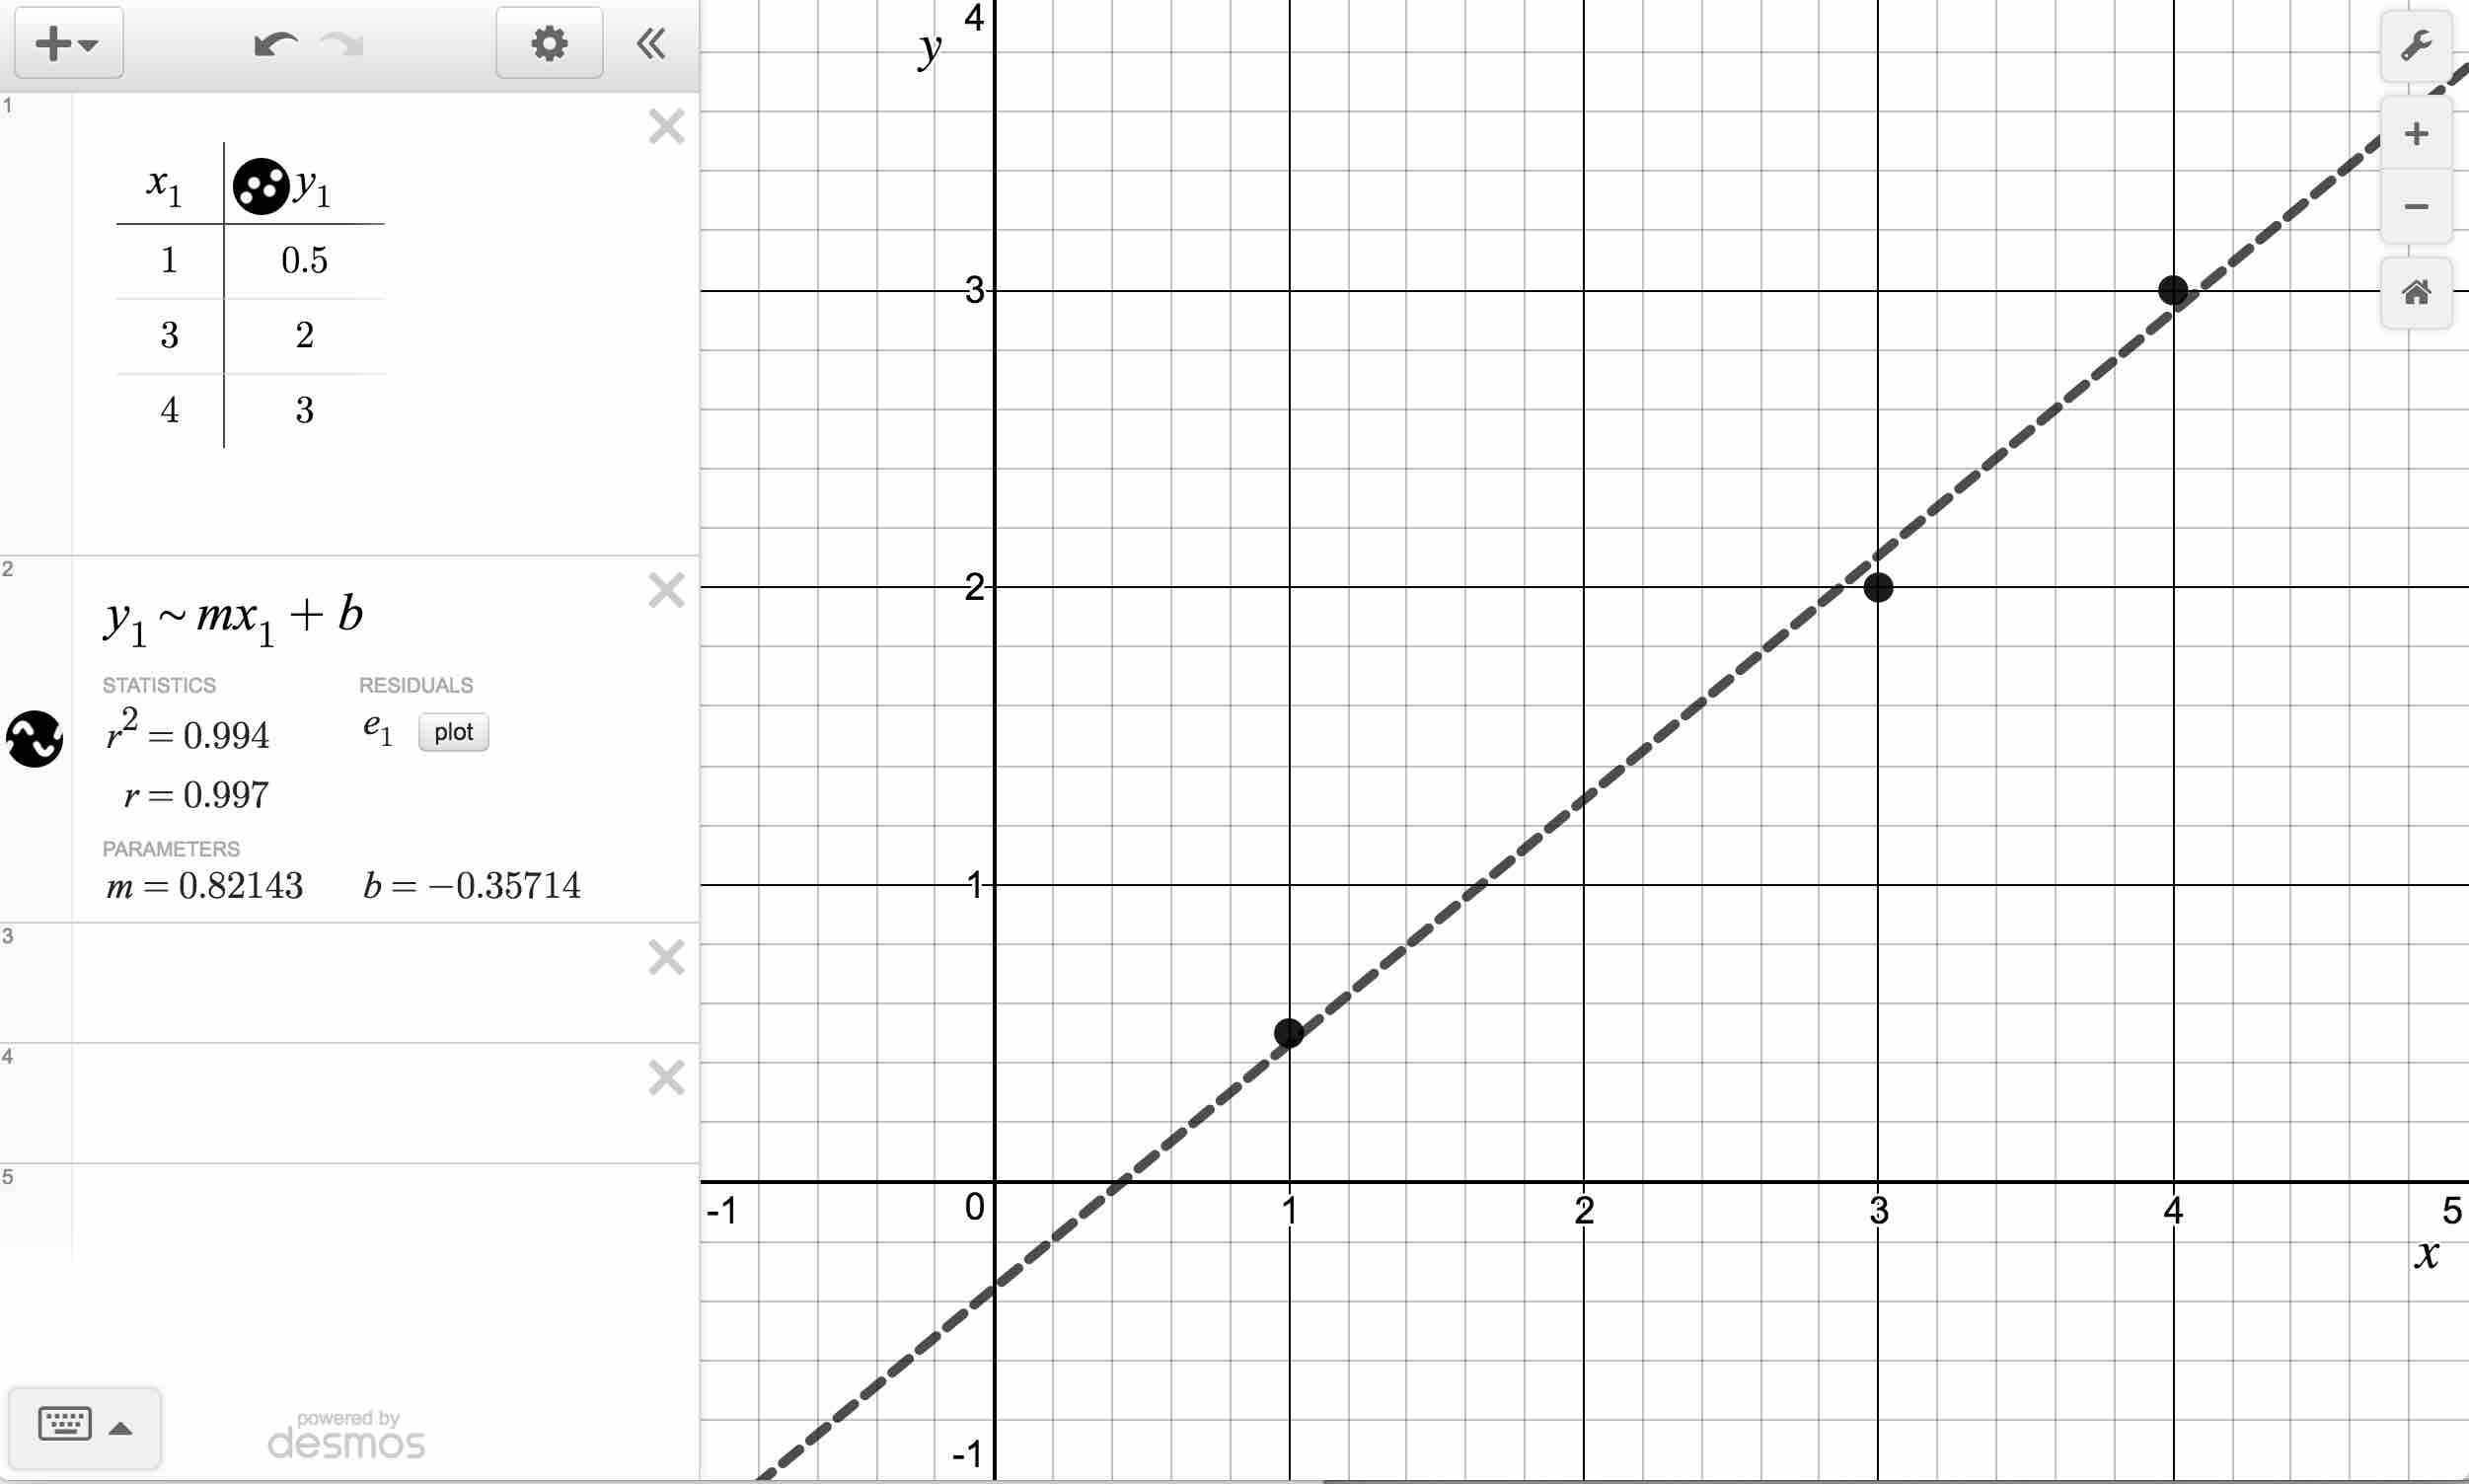
\includegraphics[width=4in]{./ConstantandLinearFunctionsGraphics/ThreePointRegression.jpg} \\
 
\end{tabular}


\enlargethispage{.25in}

Our graphing utility produces the model\footnote{We chose to use three decimal places for the approximations in this demonstration.  How many you get to use in reality varies from one application to another.} $y=mx+b$ where the slope is $m \approx 0.821$ and the $y$-coordinate of the $y$-intercept is $b \approx -0.357$.  The value $r$ is the \index{regression ! correlation coefficient}\index{correlation coefficient}\textbf{correlation coefficient} and is a measure of how close the data is to being on the same line.  The closer $|r|$ is to $1$, the better the linear fit.\footnote{The value $r^2$ is called the \index{regression ! coefficient of determination}\index{coefficient of determination}\textbf{coefficient of determination} and is also a measure of the goodness of fit. We refer the interested reader to a course in Statistics to explore the significance of $r$ and $r^2$.} Having $r \approx 0.997$ tells us that the points have a strong, positive correlation - that is, they are very close to being on a line with a positive slope, namely $y = 0.821x - 0.357$.   Indeed, the total squared error between our data set and this line is $E \approx 0.018$. The mathematics tells us that this is the smallest we can get $E$ by modifying the parameters $m$ and $b$, even though none of the data points actually lie on the line.  



Now that we have this new mathematical machinery, let's revisit Skippy's time and temperature data.
  
\begin{example} \label{timetempregressionex}  $~$
  
\begin{enumerate}
  
\item Use a graphing utility to find best fit linear models for each of the data sets below. Comment on the fit and interpret the slope of each.

\begin{center}
  
\begin{multicols}{2}
  
$\begin{array}{|c||c|}  \hline

 \text{$t$: hours after 6 a.m.}  & \text{$T$: temperature $^{\circ}$F} \\ \hline
 0 & 64  \\  \hline
 2 & 67  \\  \hline
 4 &  75  \\  \hline
 6 &  80 \\  \hline
 8 & 83  \\  \hline

\end{array}$
  

	
$\begin{array}{|c||c|}  \hline

 \text{$t$: hours after 6 a.m.}  & \text{$T$: temperature $^{\circ}$F} \\ \hline

 8 & 83  \\  \hline
 10 &  83 \\  \hline
 12 & 82  \\  \hline

\end{array}$ 
  
\end{multicols}
  
\end{center}

\item  Use your models to predict the temperature at $7$ a.m. and $3$ p.m., rounded to one decimal place.
  
\end{enumerate}

\pagebreak

{\bf Solution.}
  
\begin{enumerate}
  
 \item For our first set of data, we get the line $T = F(t) = 2.55t + 63.6$.  The value $r = 0.987$ tells us that it is a fairly good fit and we see this graphically, too.\footnote{We use $F$ as the name of the function here to distinguish it from $f$ - the function determined solely by the given set of data.}   Thus we can be confident in using this model to predict the temperature during between the hours of 6 a.m. and 2 p.m. with reasonable accuracy.   



To interpret the slope, we recognize $t$ as the independent variable (input) and $T$ as the dependent variable (output), so the slope $m = \frac{\Delta T}{\Delta t}$ is the rate of change of temperature with respect to time.   In this case,  $m = 2.55$ means that the temperature is increasing (getting warmer) at a rate of $2.55^{\circ}$F per hour.  A screenshot from Desmos is given below.

\begin{center}
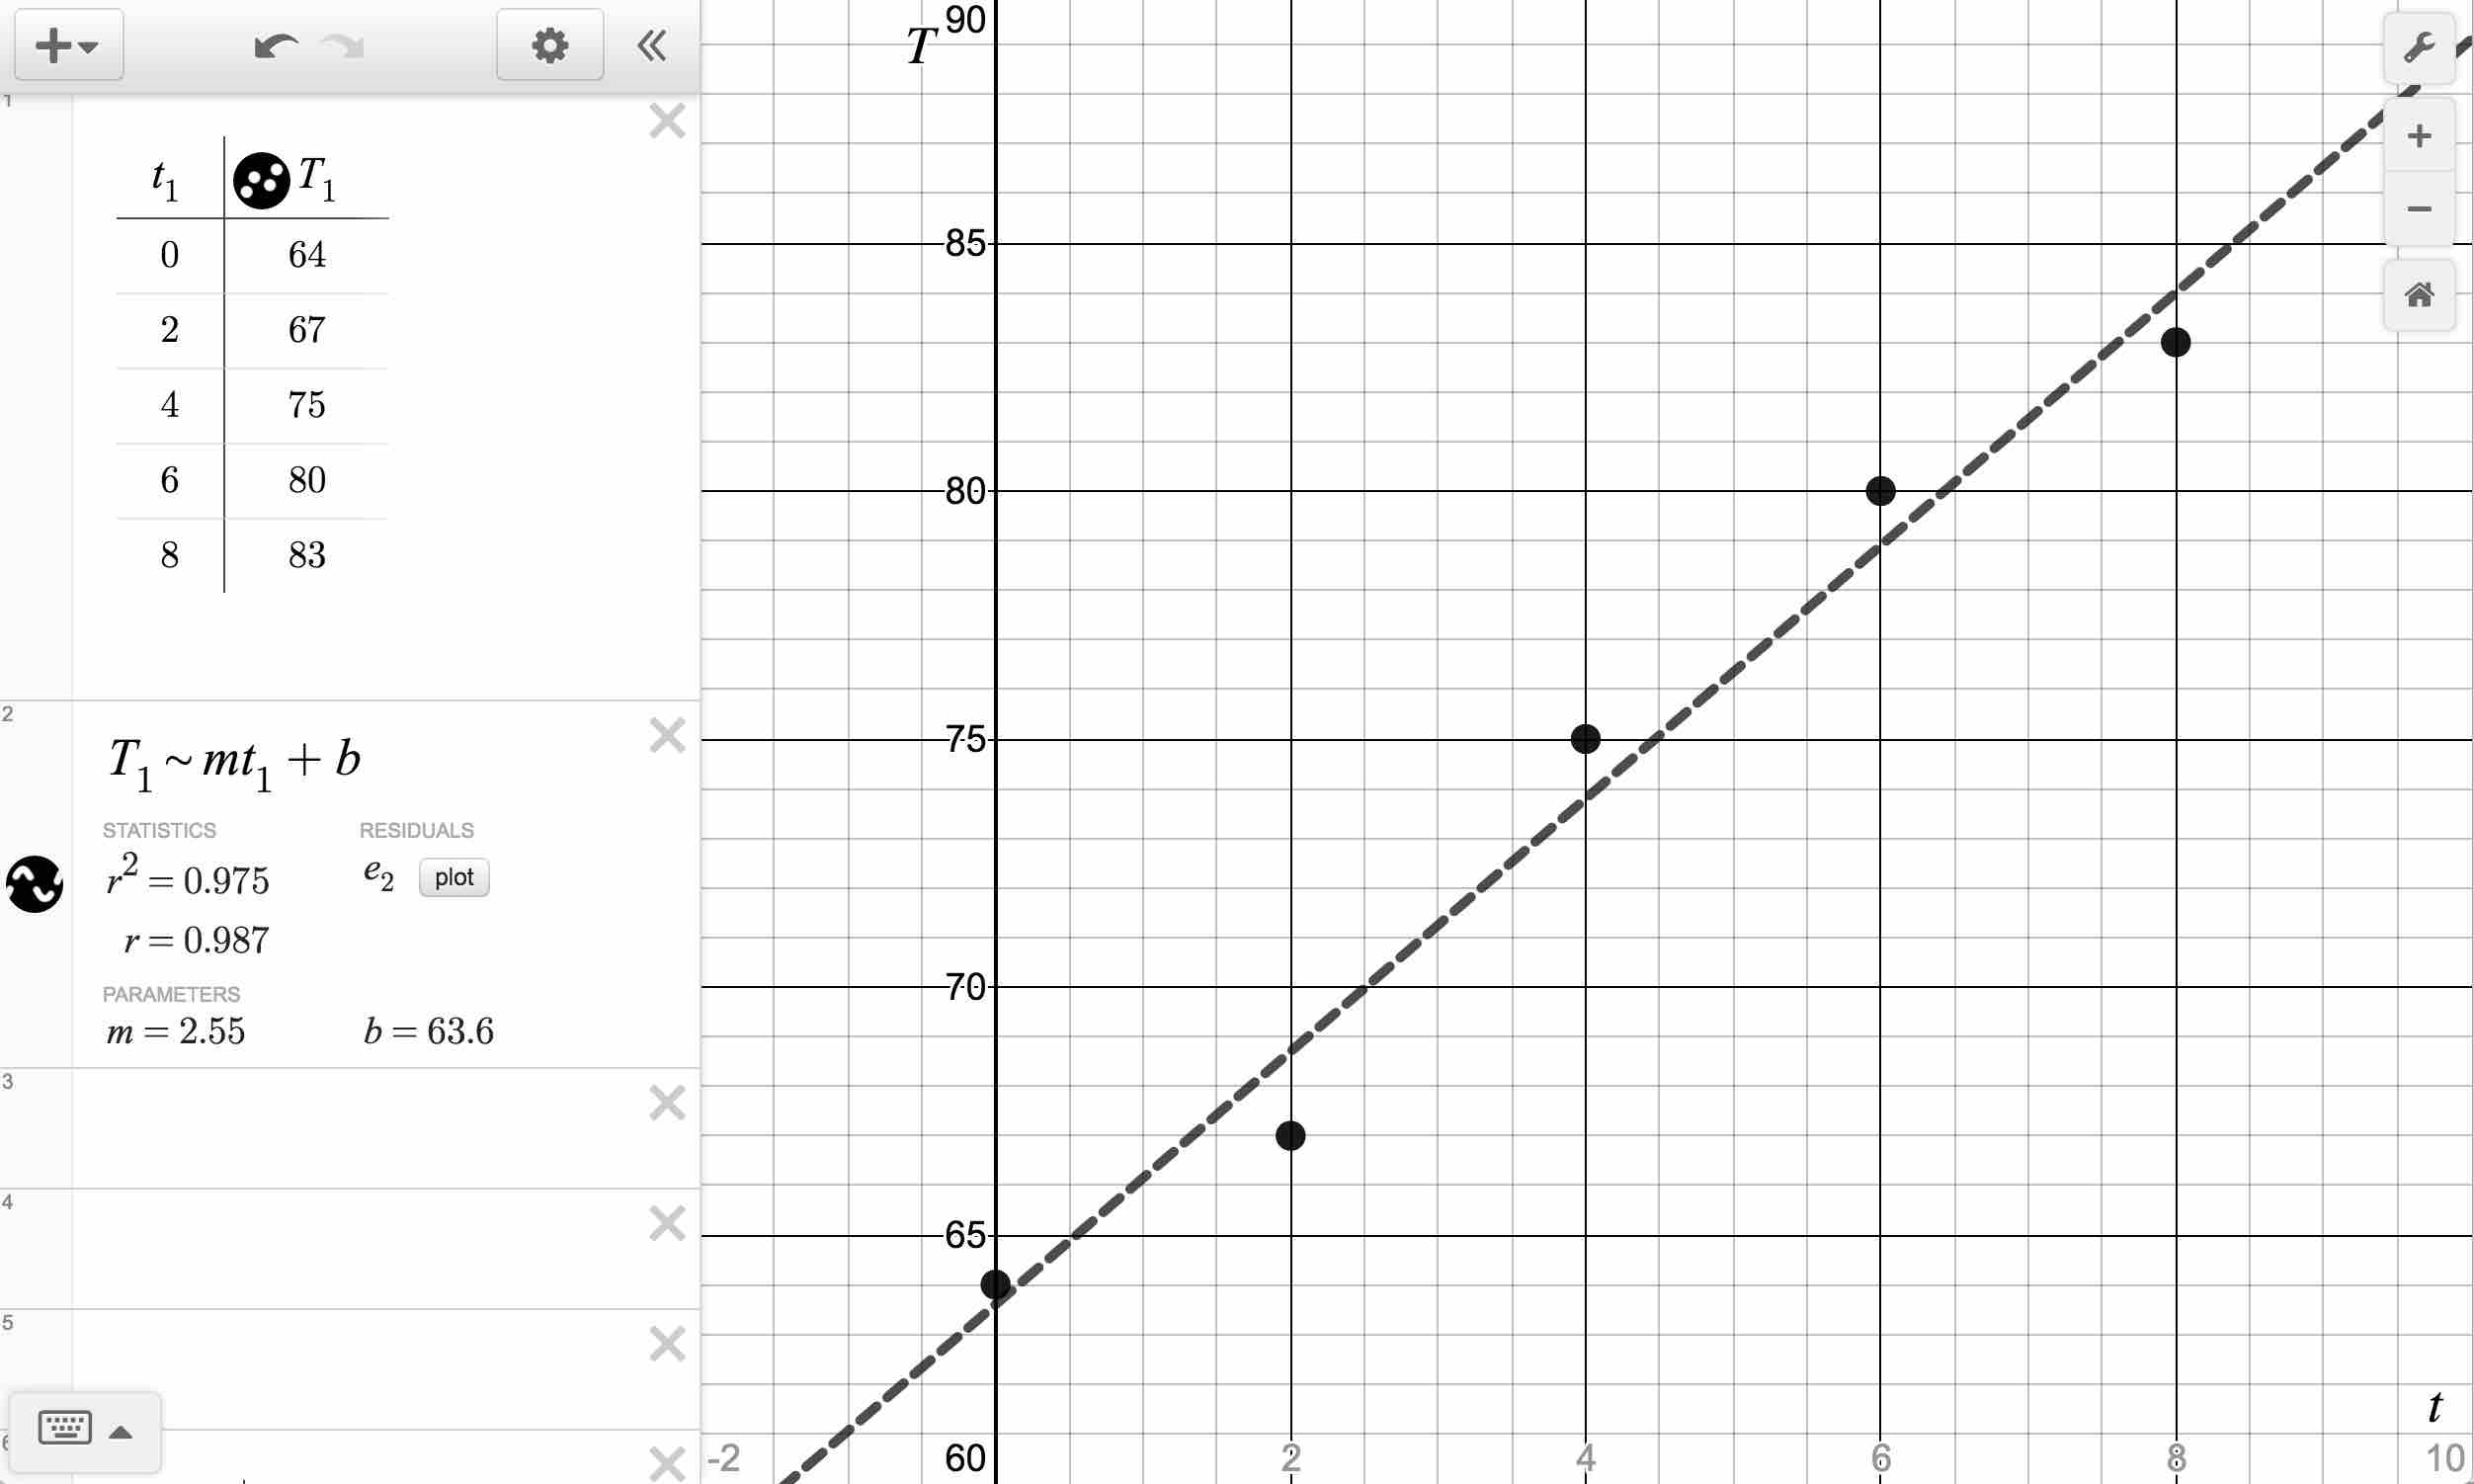
\includegraphics[width=6in]{./ConstantandLinearFunctionsGraphics/TimeTempRegression01.jpg}
\end{center}
  
For the second set of data, we get $T = G(t) = -0.25t + 85.167$ and we have $r = -0.866$.  Here, the negative sign on $r$ indicates a negative correlation which means our line has a negative slope.\footnote{We use $G$ as the function name here to distinguish it from the given function $f$ and the regression for the first data set, $F$.} While the fit looks OK, it certainly isn't as strong as with the first data set, so using this model to predict the temperature between $2$ p.m. and $6$ p.m. (let alone beyond) is a bit risky.  



The slope in this case is $m = -0.25$ which corresponds to the temperature decreasing (getting cooler) at a rate of  $0.25^{\circ}$F per hour.  That's what a negative correlation means - an increase in input (more time passes) yields a decrease in output (cooler temperatures).  As screenshot from Desmos is given at the top of the next page.
  
\begin{center}
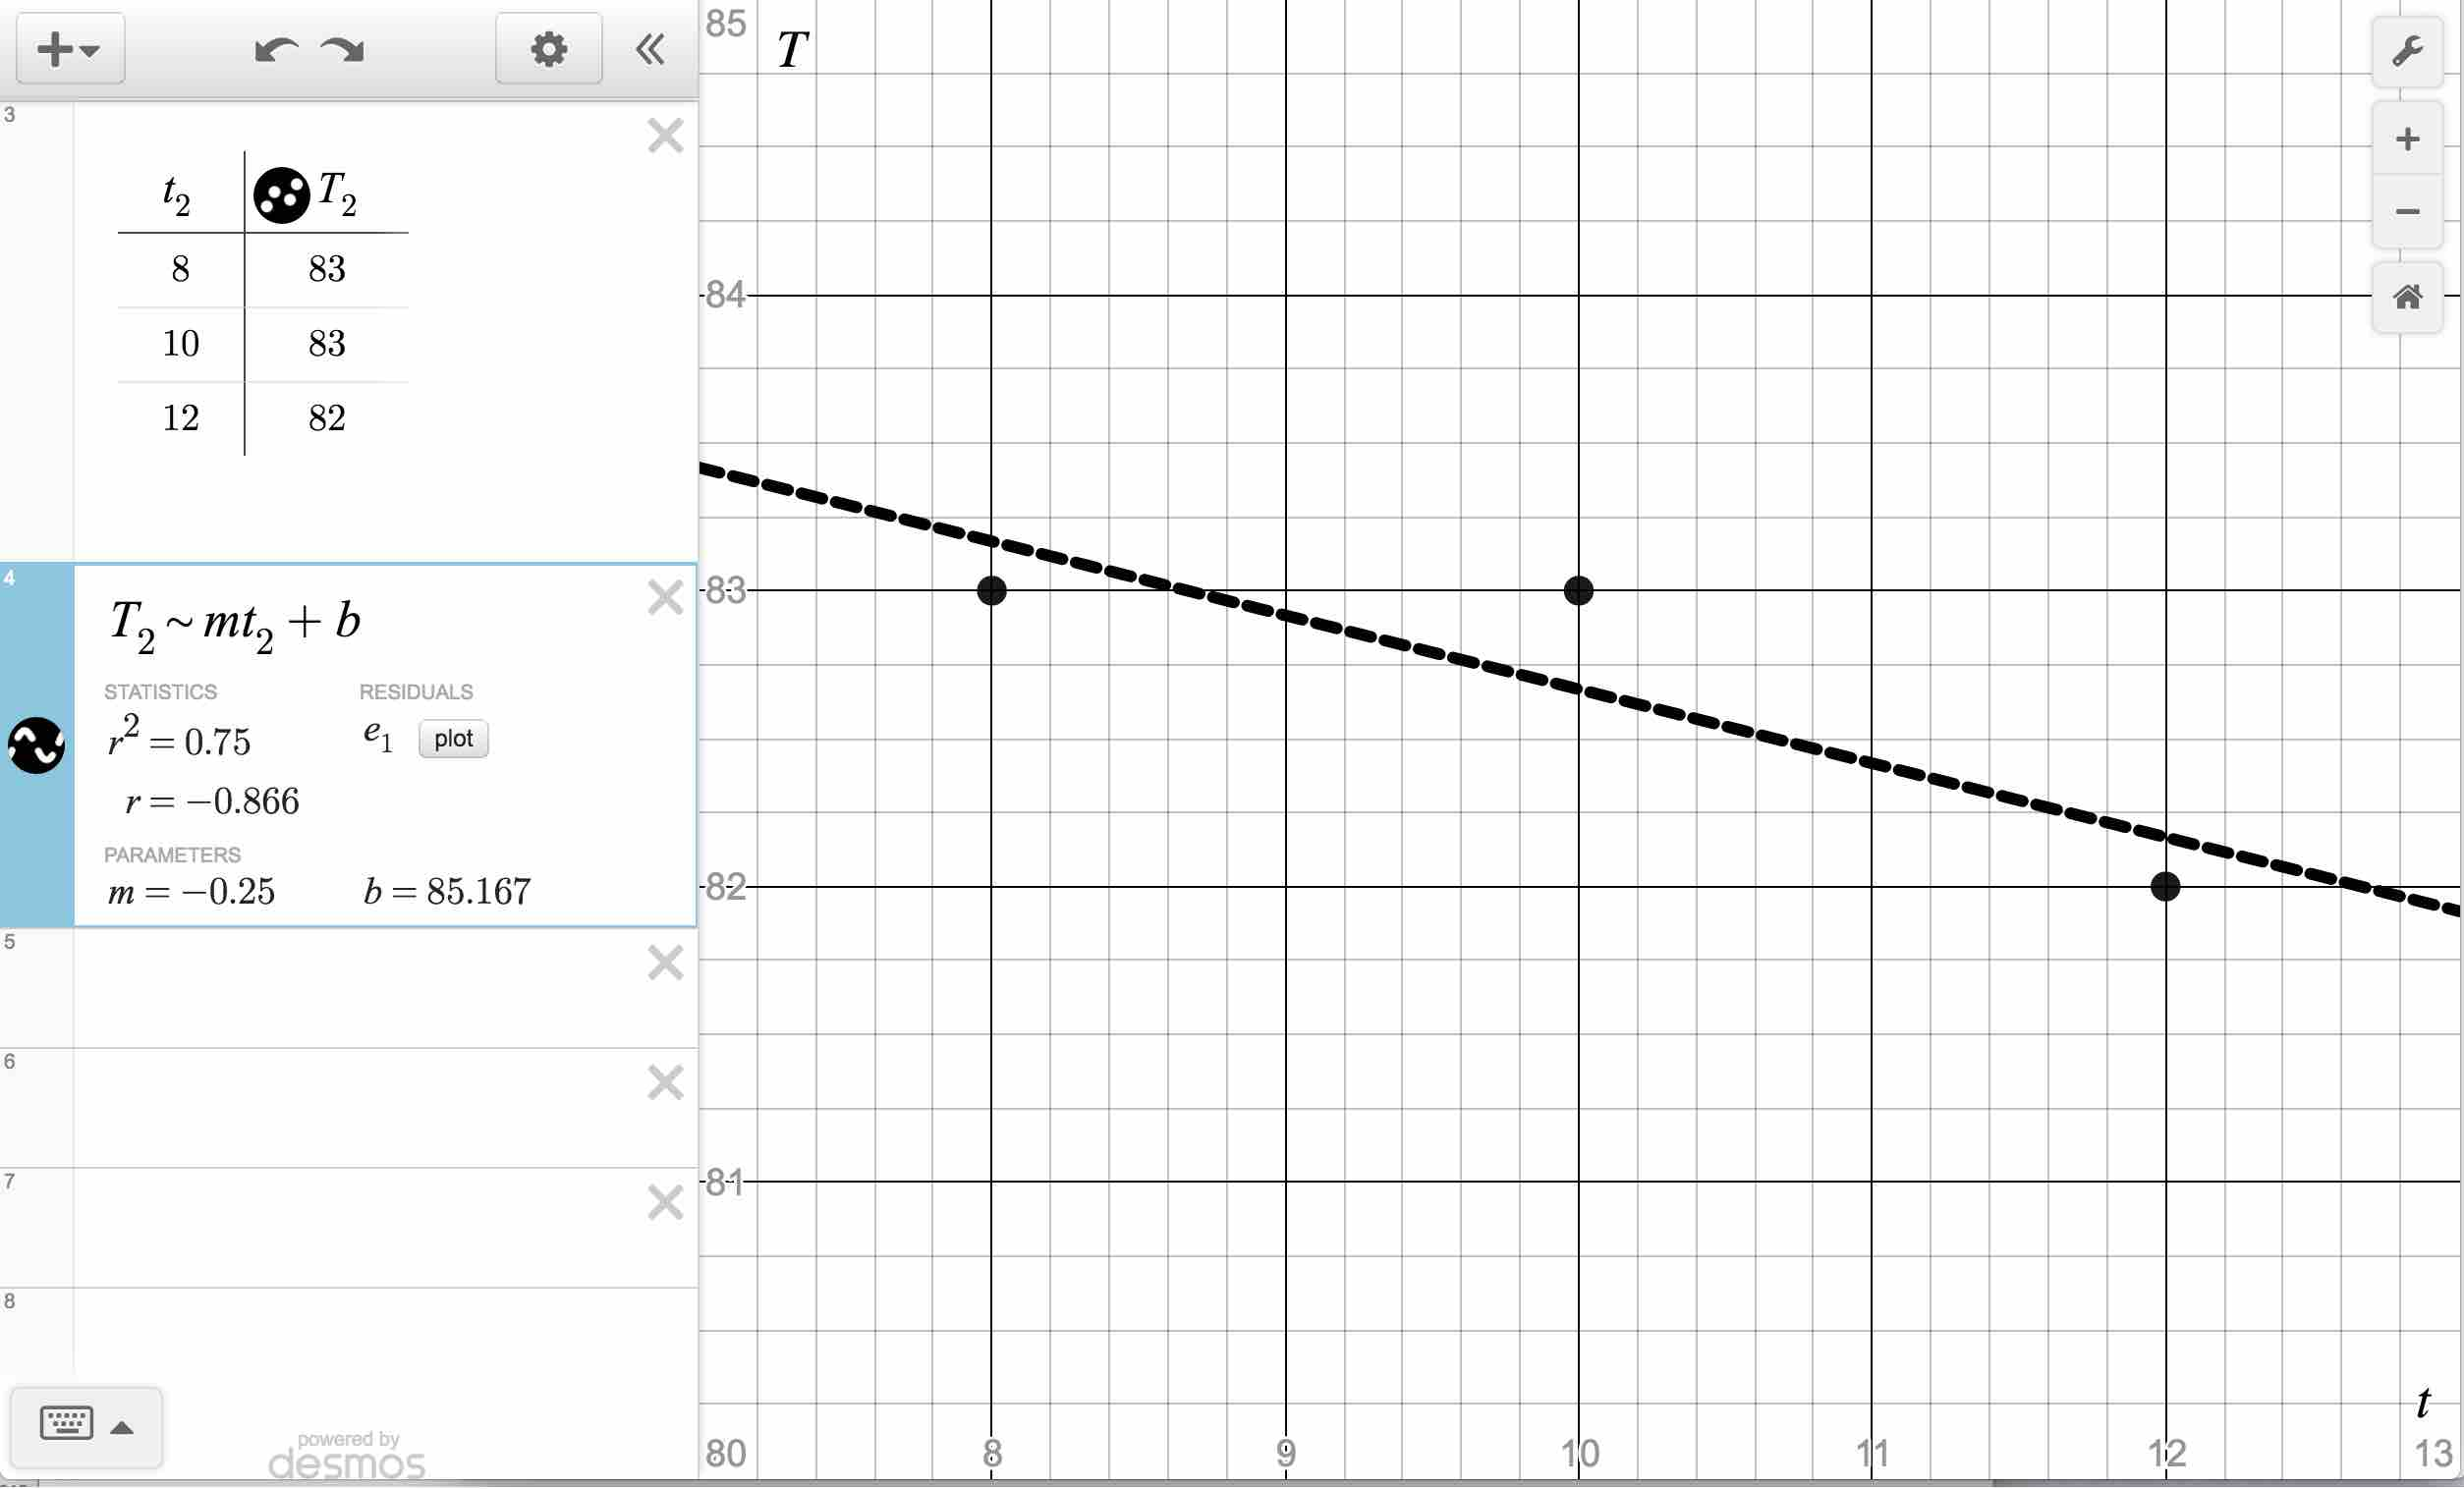
\includegraphics[width=6in]{./ConstantandLinearFunctionsGraphics/TimeTempRegression02.jpg}
\end{center}

\item  The time $7$ a.m. corresponds to $t = 1$. This falls between $t = 0$ and $t = 8$ so we use our first model.  Substituting $t = 1$ gives $T = F(1) = 2.55(1) + 63.6 \approx 66.2$.  Therefore, the model predicts the temperature to be $66.2^{\circ}$F at 7 a.m..  Likewise, $3$ p.m. corresponds to $t = 9$.  This is greater than $8$, so we use the second model: $T = G(9) =  -0.25(9) + 85.167 \approx  82.9$.  The model predicts the temperature at $3$ p.m. to be $82.9^{\circ}$F.   Based on the goodness of fit of each model, we have more confidence in the former prediction than in the latter.   \qed
  
\end{enumerate}
\end{example}
 
Examples \ref{PortaBoyCost}, \ref{PortaBoyDemand} and \ref{timetempregressionex} (among others)  represent three different levels of mathematical modeling.  In Example  \ref{PortaBoyCost},  the mathematical model (the cost function) was provided and our task was to use the model to \textbf{interpret} the mathematics in that context.    In Example  \ref{PortaBoyDemand}, we were given a minimal amount of information, namely, two data points, and then asked to \textbf{construct} a model which fit those data exactly.  Lastly, in Example \ref{timetempregressionex}, we were given several data points and we used statistical methods to construct a \textbf{best fit} model to the data. 



The validity of the models rests on the validity of the underlying assumptions used to create the models.  For instance, is there any reason to assume a price-demand function would be linear?  Is it reasonable to assume that the temperature changes at a constant rate? These are questions for economists and scientists.  Mathematicians often take on a role of equal parts translator and prophet:  they codify ideas into formulas and then use them to make predictions about yet-to-be observed phenomena.  


\subsection{The Average Rate of Change of a Function}
\label{AverageRateofChange}

As mentioned earlier in the section, the concepts of slope and the more general rates of change are important concepts not just in Mathematics, but also in other fields.   Many important phenomena are modeled using non-linear functions, and while the rates of change of these functions are not constant, we can sample the function at two points and compute what is known as an \textbf{average rate of change} between them to give some sense as to the function's behavior over that interval.\footnote{We are basically pretending that the function is linear on a short interval to see what we can say about its behavior.}



\colorbox{ResultColor}{\bbm

\begin{defn} \label{arc}  Let $f$ be a function defined on the interval $[a,b]$. 

\smallskip

 The \index{average rate of change}\index{rate of change ! average}\textbf{average rate of change}  of $f$ over $[a,b]$ is defined as: \[ \dfrac{\Delta [f(x)]}{\Delta x} = \dfrac{f(b) - f(a)}{b-a} \]

Geometrically, the average rate of change is the slope of the line\footnote{This line is called a \index{secant line}\index{line ! secant}\textbf{secant line}.}  containing $(a, f(a))$ and $(b, f(b))$.

\end{defn}

\ebm}



\begin{center}
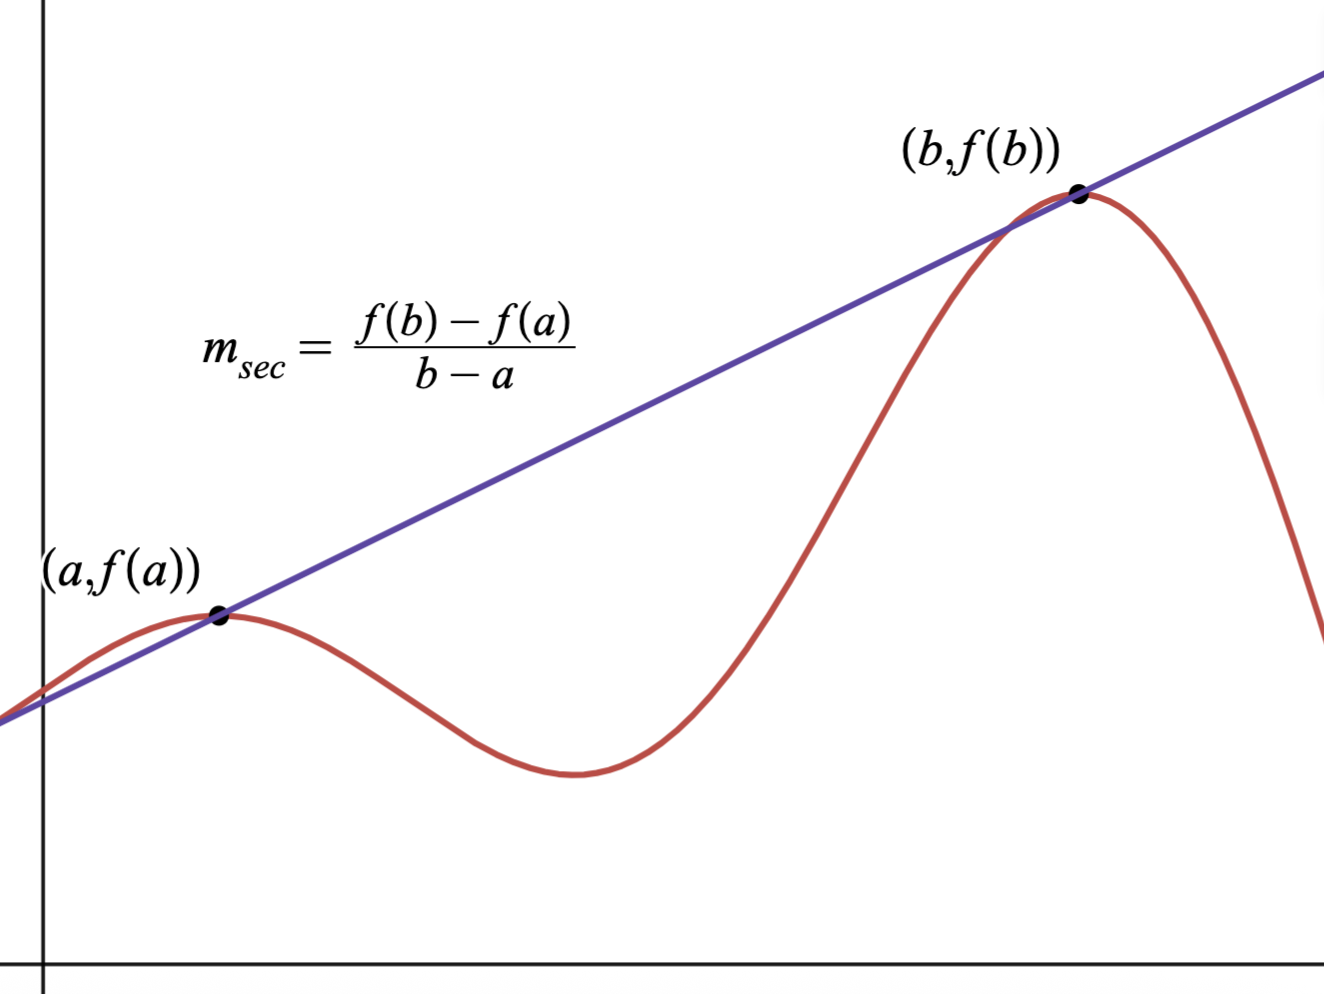
\includegraphics[width=4in]{./ConstantandLinearFunctionsGraphics/SecantLine.png}

The graph of a function $f$ along with the secant line through the points $(a, f(a))$ and $(b, f(b))$.

\end{center}

As with Definitions \ref{absmaxmindefn}  and \ref{incdeccnstdefn}, the wording in Definition \ref{arc}, while referring to the function $f$, is really making a statement about its outputs $f(x)$.  



If $f$ is increasing over $[a,b]$, then the average rate of change will be positive. Likewise, if $f$ is decreasing or constant, the average rate of change will be negative or $0$, respectively. (Think about this for a moment.) However, as the next example demonstrates, the converses of these statements aren't always true.\footnote{For example, the average rate of change over an interval could be positive yet the function could decrease over part of that interval and then increase on a different part.}

\begin{example} \label{ARCRocketExample} The formula $s(t) = -5t^{\,2} + 100t$ for $0 \leq t \leq 20$ gives the height, $s(t)$, measured in feet, of a model rocket above the Moon's surface as a function of the time $t$, in seconds after lift-off.

\begin{enumerate}

\item Find $s(0)$, $s(5)$, $s(10)$, $s(15)$ and $s(20)$ and use these along with a graphing utility to graph $y = s(t)$.

\item State the range of $s$ and interpret the extrema, if any exist.

\item Find and interpret the $t$- and $y$-intercepts.  

\item Find and interpret the interval(s) over which $s$ is increasing, decreasing or constant.  

\item Find and interpret the average rate of change of $s$ over the intervals $[0,5]$, $[5,10]$, $[10, 20]$ and $[5, 15]$.


\end{enumerate}

{\bf Solution.}

\begin{enumerate}

\item  To find $s(0)$, we substitute $t=0$ into the formula for $s(t)$:  $s(0) = -5(0)^2+100(0) = 0$.  Similarly,  $s(5) = -5(5)^2+100(5) = -5(25)+500 = -125+500 = 375$.  Continuing, we obtain: $s(10) = 500$, $s(15) = 375$ and $s(20) = 0$.  We construct a table of values and with a graphing utility we obtain:

\begin{center}
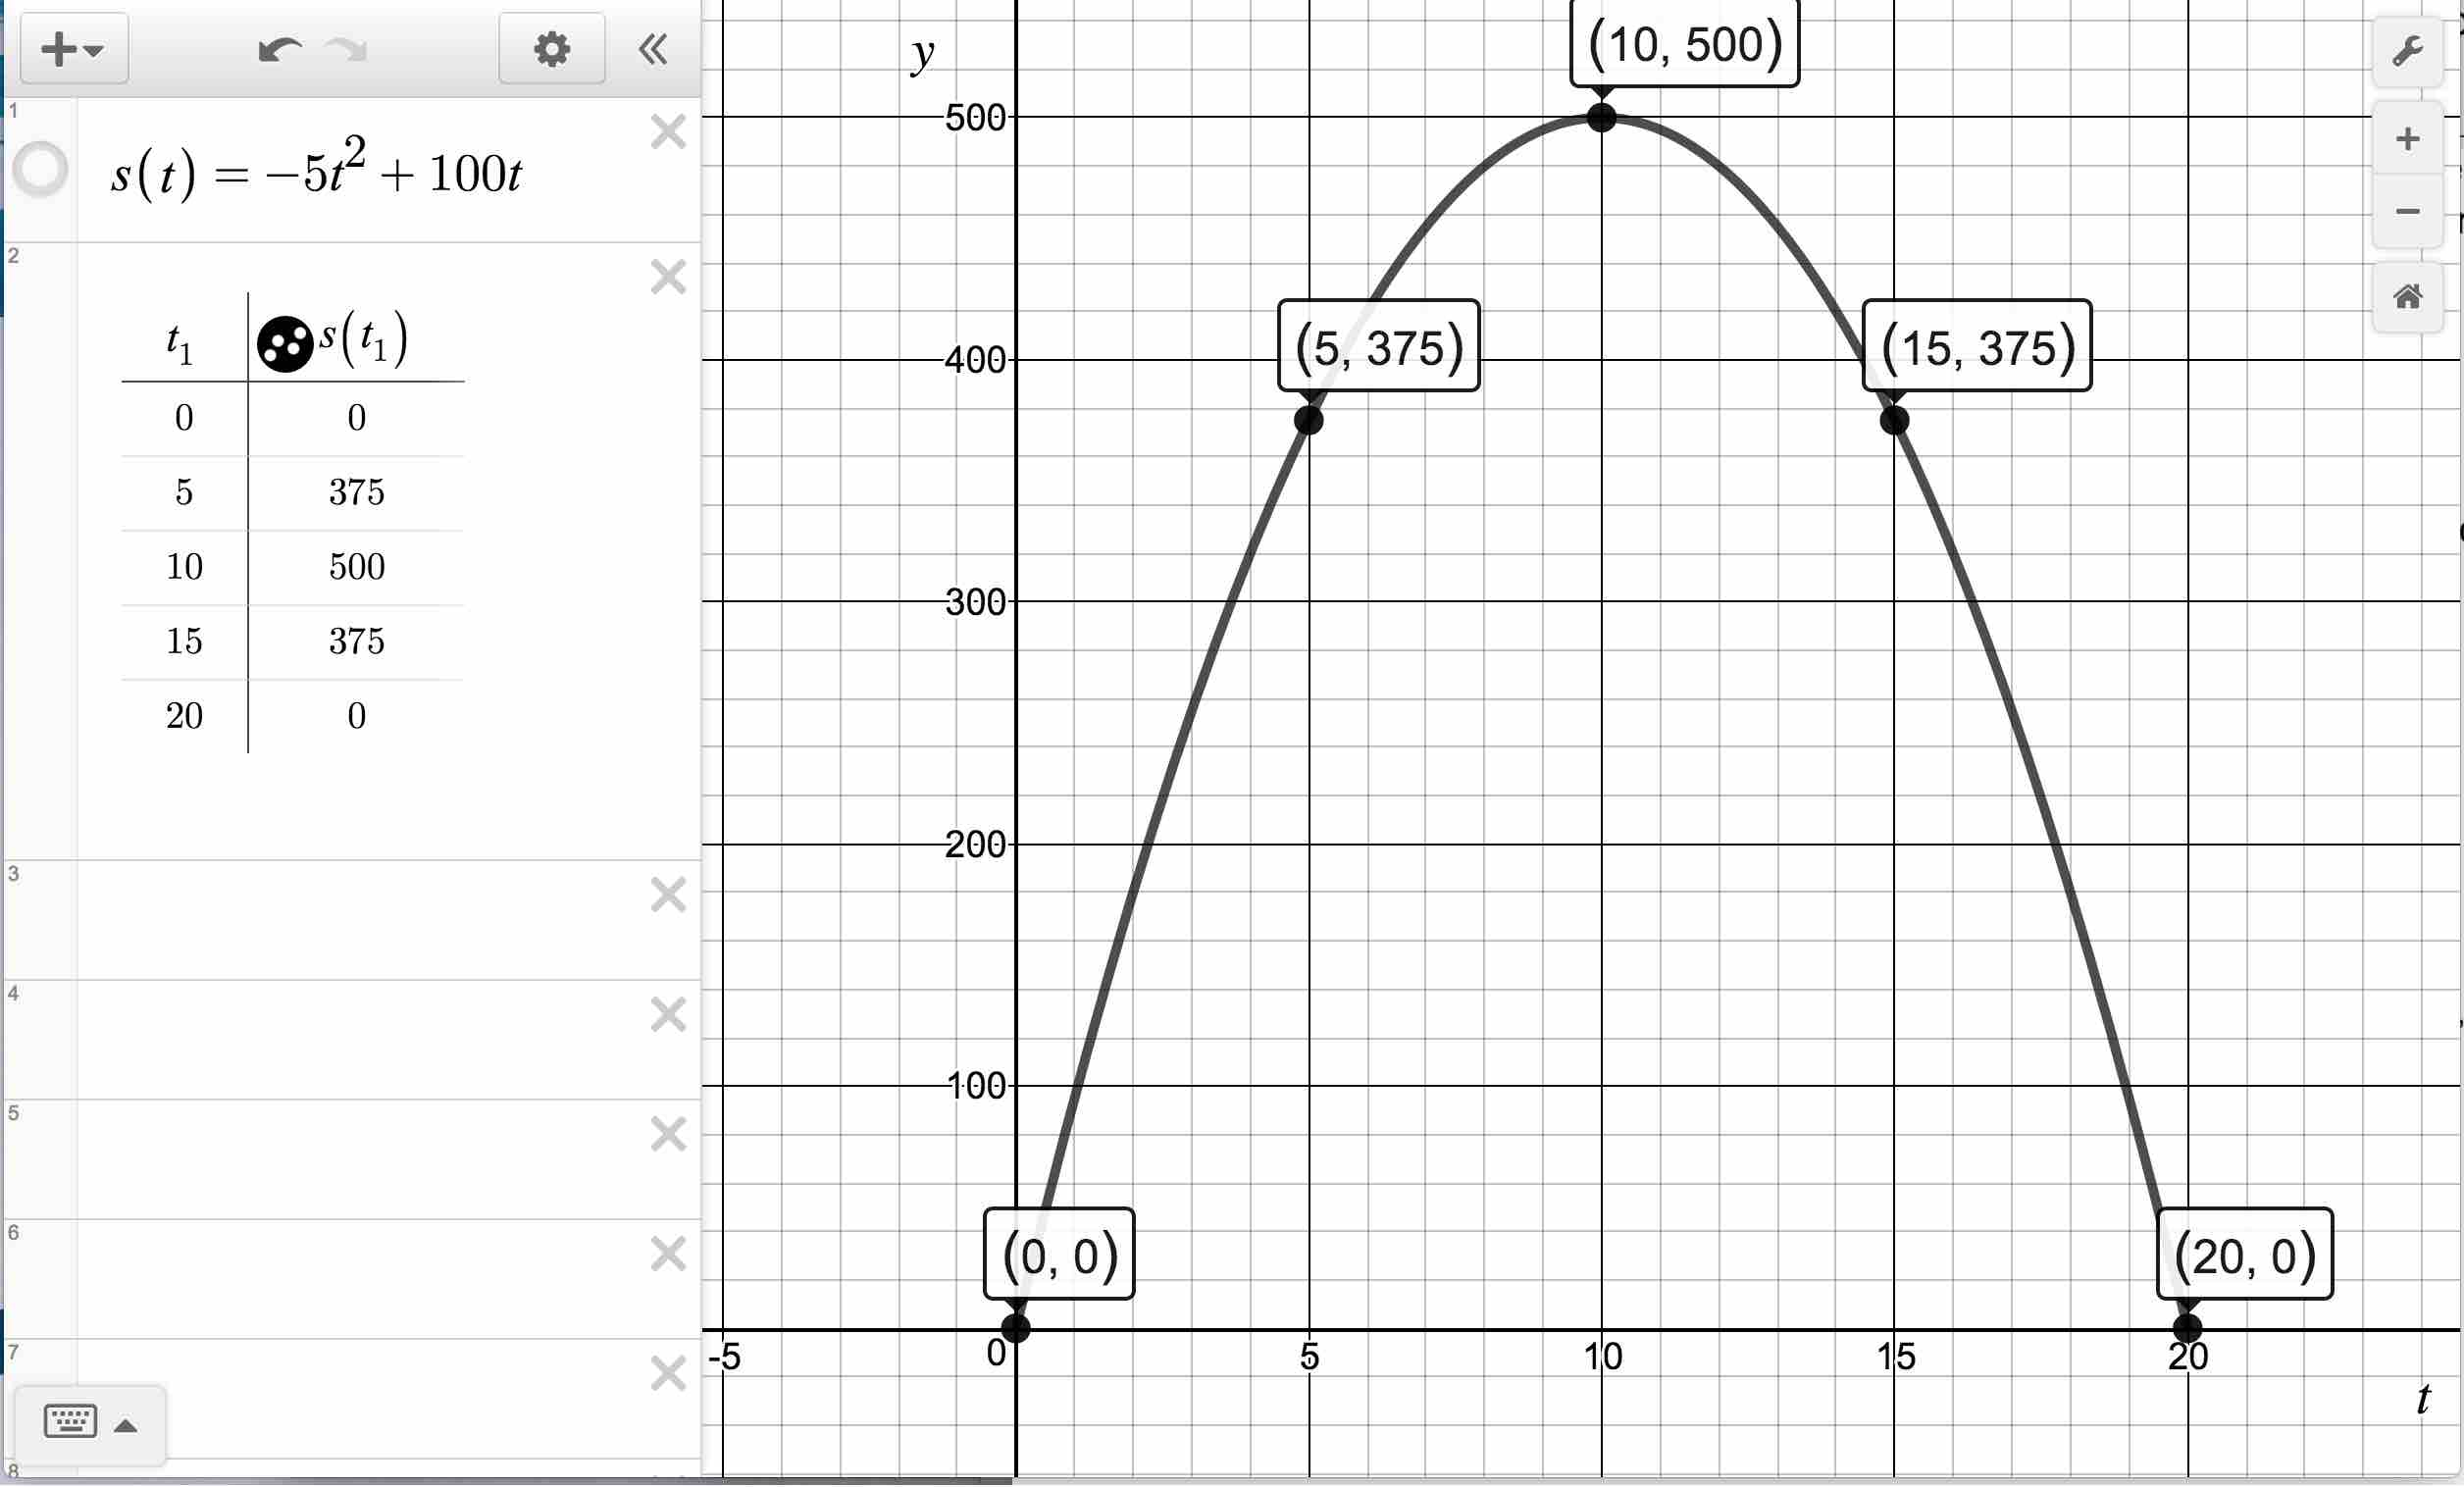
\includegraphics[width=6in]{./ConstantandLinearFunctionsGraphics/ARCRocketExample01.jpg}

\end{center}

\item  Projecting the graph to the $y$-axis, we see that the range of $s$ is $[0, 500]$ so the minimum of $s$ is $0$ and the maximum is $500$.  This means that the rocket at some point is on the surface of the Moon and reaches its highest altitude of $500$ feet above the lunar surface.

\item The first intercept we see is $(0, 0)$ which is both a $t$- and a $y$-intercept.  Since $t$ is the time after lift-off and $y = s(t)$ is  the height above the Moon's surface, the point $(0, 0)$ means that the model rocket was launched ($t=0$) from the Moon's surface ($s(t) = 0$).  The remaining intercept, $(20, 0)$,  is another $t$-intercept.  This means that $20$ seconds after lift-off ($t=20$), the model rocket returns to the Moon's surface ($s(t) = 0$).   That is, the `time of flight' of the model rocket is 20 seconds.

\item  Referring to Definition \ref{incdeccnstdefn}, $s$ increases over the interval $[0, 10]$, since for those values of $t$, as we read from left to right, the graph of the function is rising meaning the $y$ values (hence $s(t)$ values) are getting larger. Thus the model rocket is heading upwards for the first $10$ seconds of its flight.  We find that $s$ decreases over the interval $[10, 20]$, indicating once it has reached its highest altitude of $500$ feet $10$ seconds into the flight, the rocket begins to fall back to the surface of the Moon, landing $20$ seconds after lift-off.

\item  To find the average rate of change of $s$ over the interval $[0, 5]$ we compute \[ \dfrac{\Delta[s(t)]}{\Delta t} = \dfrac{s(5) - s(0)}{5 - 0} = \dfrac{\text{$375$ feet}}{\text{$5$ seconds}} = \text{$75$ feet per second}.\] In other words, the height is \textbf{increasing} at an \textbf{average rate} of $75$ feet per second during the first 5 seconds of flight.  The rate here is called the\index{average velocity} \index{velocity ! average} \textbf{average velocity} of the rocket over this interval.  Velocity differs from speed in that velocity comes with a direction.  In this case, a positive velocity indicates that the rocket is traveling \textbf{upwards}, since when $s$ is increasing, the model rocket is climbing higher.  



Similarly, the average rate of change of $s$ over the interval $[5, 10]$ works out to be $25$.  This means that the average velocity over the next $5$ seconds of the flight has slowed to $25$ feet per second. The model rocket is still, on average, traveling upwards, albeit more slowly than before.  



Over the interval $[10, 20]$, the average rate of change of $s$ works out to be $-50$.  This means that, on average, the rocket is \textbf{falling} at a rate of $50$ feet per second.  The rocket has managed to fall from its highest point $500$ feet above the surface of the Moon back to the Moon's surface in $10$ seconds so this makes sense. Finally, the average rate of change of $s$ over $[5, 15]$ is $0$.  This means that the model is the same height above the ground after $5$ seconds ($375$ feet) as it is after $15$ seconds.    



Geometrically, the average rate of change of a function over an interval can be interpreted as the slope of a secant line. Below on the left is a dotted line containing $(0, 0)$ and $(5, 375)$ (which has slope $75$) along with a dotted line containing the points $(5, 375)$ and $(10, 500)$ (which has slope $25$).  Visually, the lines help demonstrate that, while $s$ is increasing over $[0, 10]$, the rate of increase is slowing down as $t$ nears $10$.  



\begin{multicols}{2}


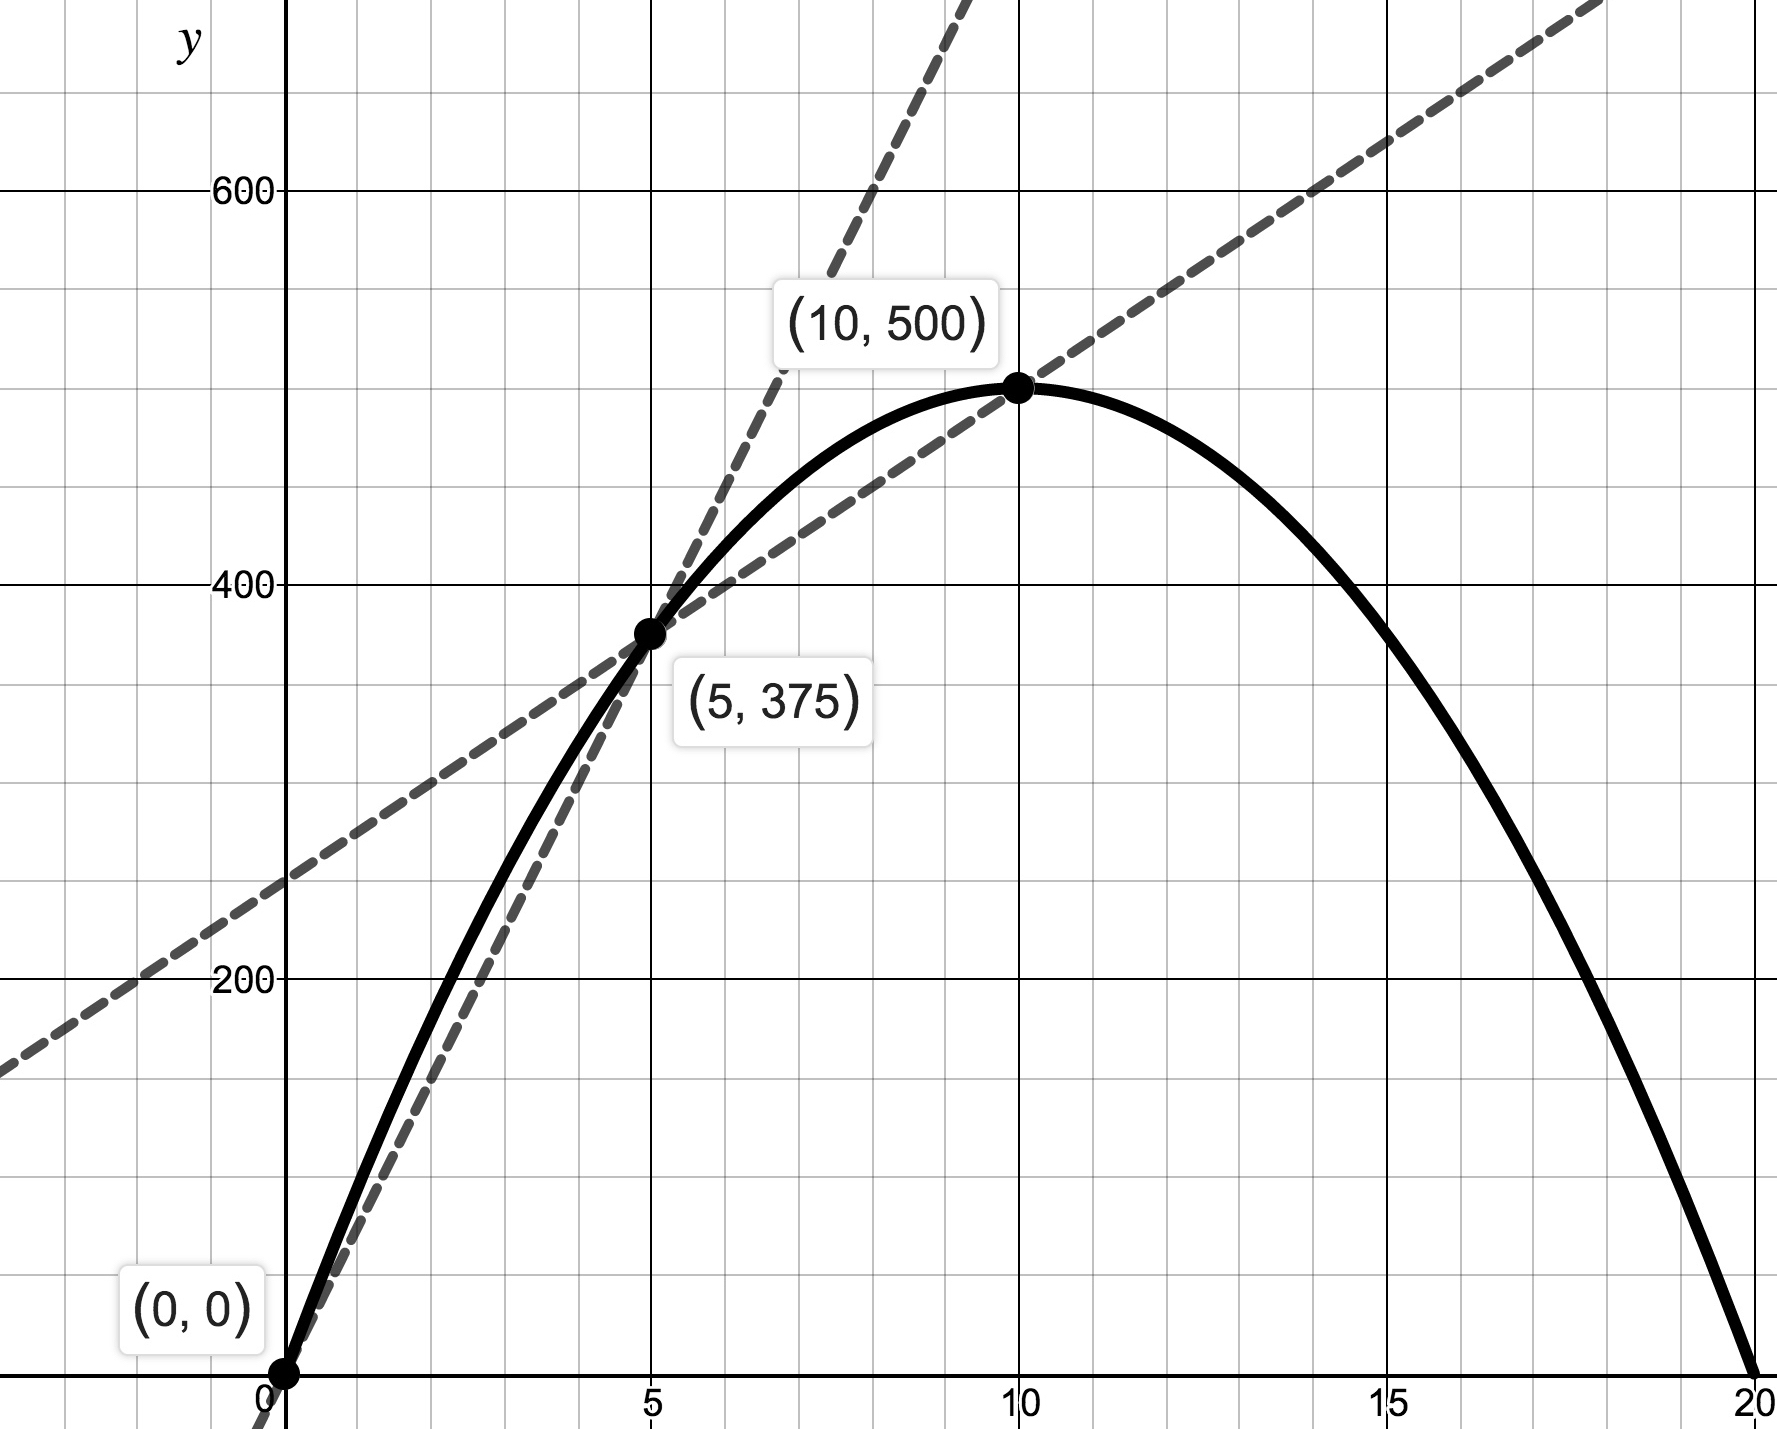
\includegraphics[width=2.75in]{./ConstantandLinearFunctionsGraphics/ARCRocketExample02.jpg}

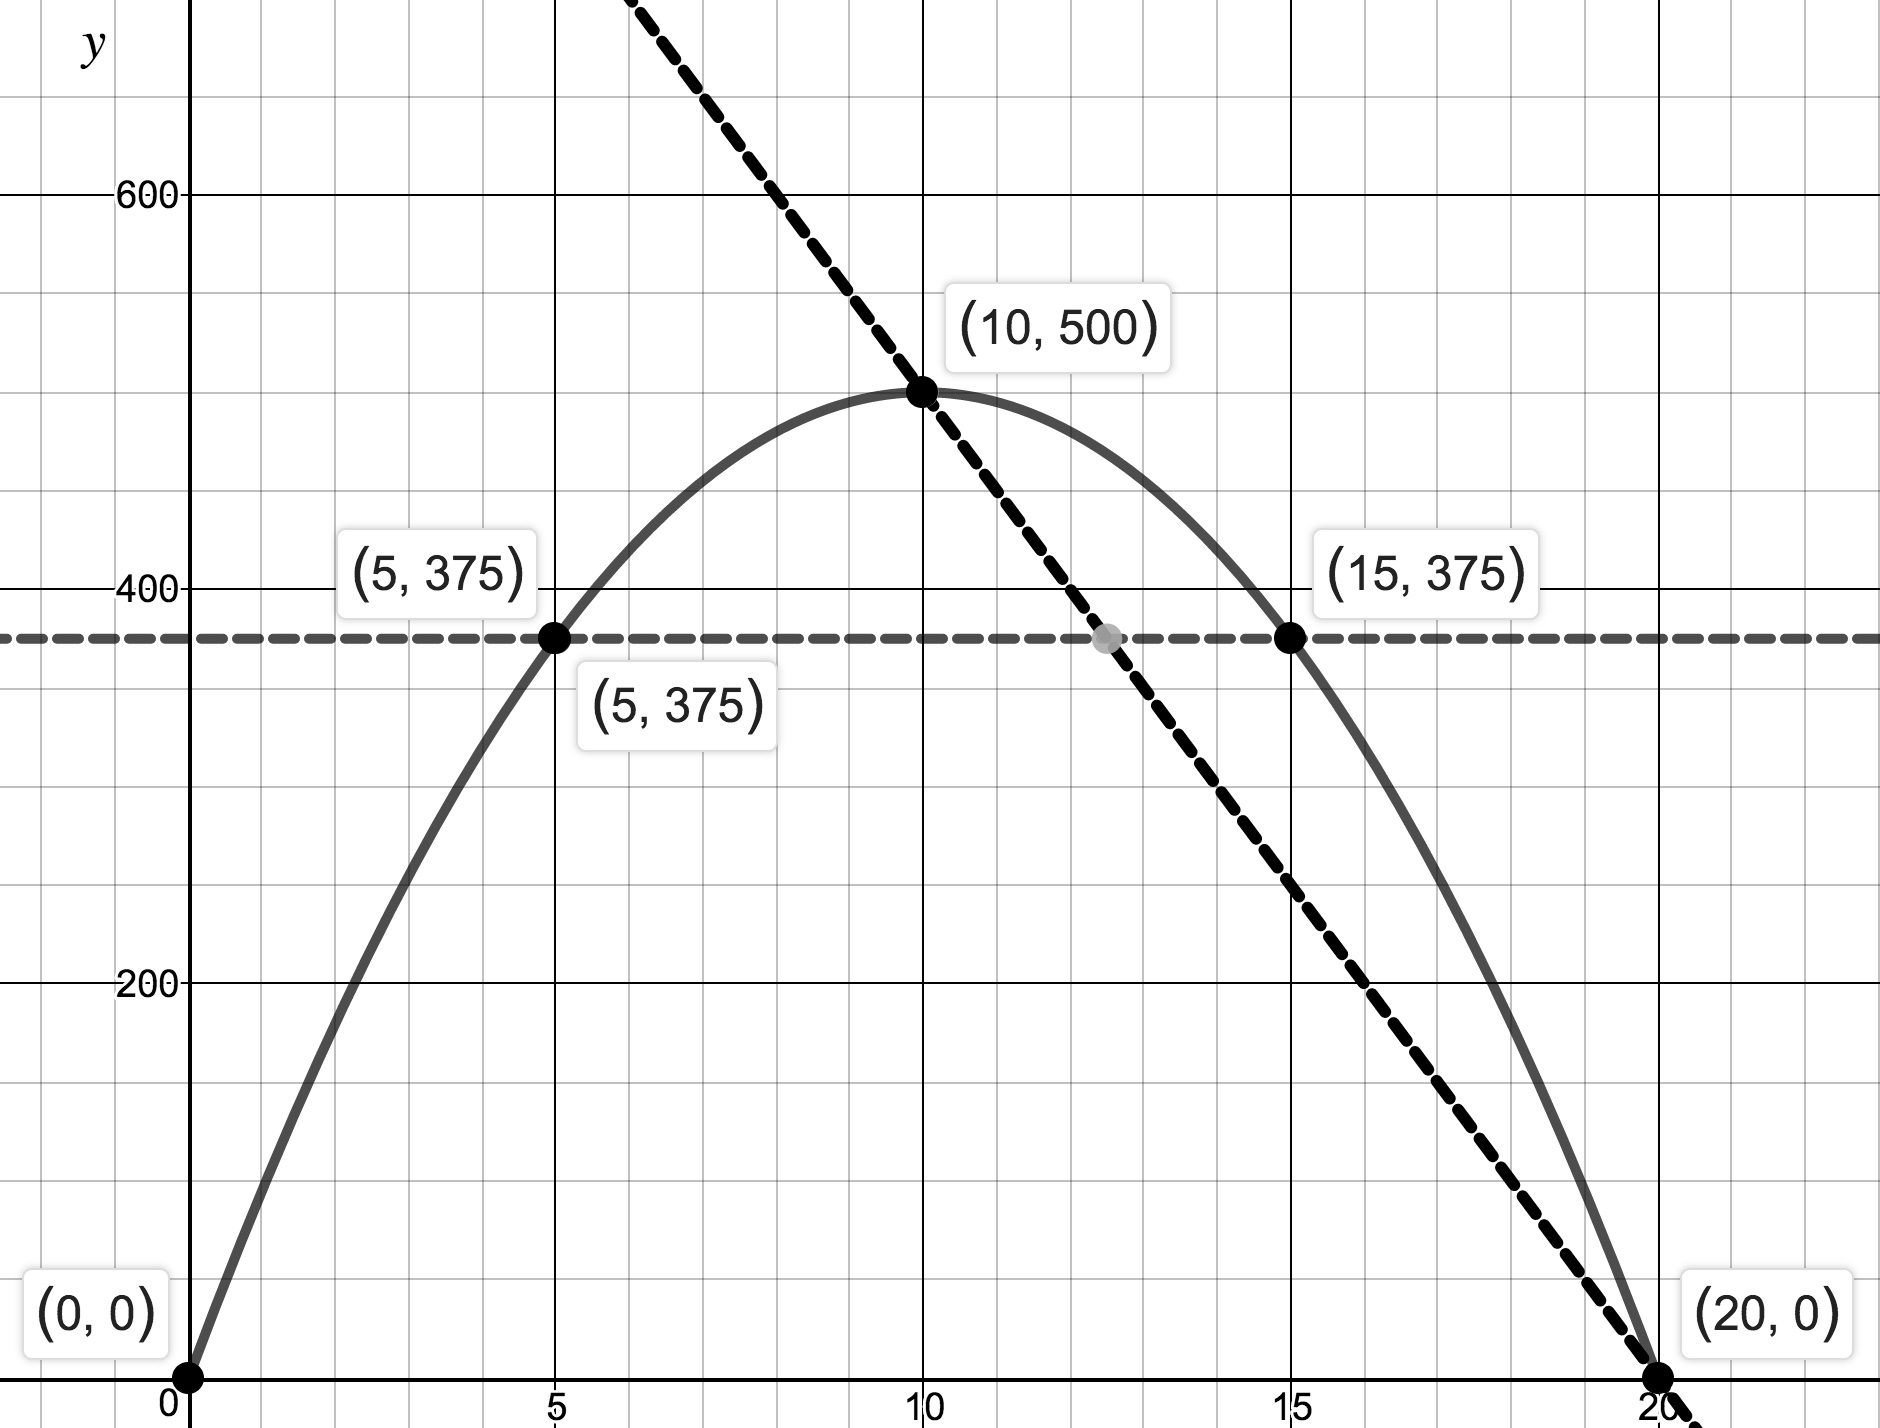
\includegraphics[width=2.75in]{./ConstantandLinearFunctionsGraphics/ARCRocketExample03.jpg}


\end{multicols}


The graph above on the right depicts a dotted line through $(10, 500)$ and $(20,0)$ indicating a net decrease over that interval.  We also have a horizontal line ($0$ slope) containing the points $(5, 375)$ and $(15, 375)$, which shows no net change between those two points, despite the fact that the rocket rose to its maximum height then began its descent during the interval $[5, 15]$.   \qed




\end{enumerate}



\end{example}

An important lesson from the last example is that average rates of change give us a snapshot of what is happening \textbf{at the endpoints} of an interval, but not necessarily what happens \textbf{over the course} of the interval.  Calculus gives us tools to compute slopes \textbf{at} points which correspond to  \textbf{instantaneous} rates of changes.  While we don't quite have the machinery to properly express these ideas, we can hint at them in the Exercises. Speaking of exercises \ldots 

\end{document}
